\documentclass[12pt]{article}

\usepackage[ngerman]{babel}
\usepackage{titlesec}
\usepackage{graphicx}
\usepackage{textcomp}
\usepackage[a4paper, lmargin=2.5cm, rmargin=2.5cm, top=2.5cm, bottom=3cm]{geometry}
\usepackage{setspace}
\usepackage{amsfonts}
\usepackage[utf8]{inputenc}
\usepackage{stmaryrd}
\usepackage{bibgerm}
\usepackage{caption}
\usepackage{aligned-overset}
\usepackage{subcaption}
\usepackage[utf8]{inputenc}
\pagestyle{plain}
\pagenumbering{arabic}
%\usepackage[square,sort,comma,numbers]{natbib}
\usepackage{pifont}
\usepackage{array}

\newcommand{\cmark}{\ding{51}}%
\newcommand{\xmark}{\ding{55}}%

\usepackage{amsmath,amssymb,amstext,mathtools,amsthm,amsfonts}
\usepackage{xcolor}
\usepackage[ngerman]{babel}
\usepackage{booktabs}
%\usepackage{chemformula} % Für die chemische Formel
\usepackage{graphicx}
\usepackage{caption}
\usepackage{bigints}
\usepackage{bm}
%\usepackage{makecell}
%\newcommand{\abs}[1]{{\left| #1 \right|}}
%\renewcommand\theadalign{bc}
%\renewcommand\theadfont{\bfseries}
%\renewcommand\theadgape{\Gape[4pt]}
%\renewcommand\cellgape{\Gape[4pt]}

\usepackage{xcolor}
\usepackage[framemethod,tikz]{mdframed}
\usetikzlibrary{shadows}

\mdfdefinestyle{outer}{outerlinewidth=0.5pt,backgroundcolor=blue!5,roundcorner=10pt,outerlinecolor=blue,innerlinewidth=0.5pt,innerlinecolor=black}
\mdfdefinestyle{inner}{leftmargin=0.1cm,rightmargin=0.1cm,outerlinewidth=0.5pt,innerlinewidth=0.5pt,innerlinecolor=black,outerlinecolor=black,backgroundcolor=lightgray!10,roundcorner=5pt,linecolor=black}

\newcommand{\qenc}{q_{\boldsymbol\phi}(\mathbf{z}|\mathbf{x}_i)}
\newcommand{\qencd}{q_{\phi}(z|x_i}
\newcommand{\penc}{p_{\boldsymbol\theta}(\mathbf{z}|\mathbf{x}_i)}
\newcommand{\pdec}{p_{\boldsymbol\theta}(\mathbf{x}_i|\mathbf{z})}
\newcommand{\E}{\mathbb{E}}
\newcommand{\R}{\mathbb{R}}
\newcommand{\tx}{\widetilde{x}}
\newcommand{\tz}{\widetilde{z}}
\newcommand{\tZ}{\widetilde{Z}}
\newcommand{\tX}{\widetilde{X}}
\newcommand{\tmu}{\widetilde{\mu}}
\newcommand{\tsig}{\widetilde{\sigma}}
\newcommand{\bP}{\mathbb{P}}
\newcommand{\bbf}{\bold{f}}
\newcommand{\bmu}{\bm{\mu}}
\newcommand{\bsig}{\bm{\sigma}}
\newcommand{\N}{\mathbb{N}}
\newcommand{\z}{\mathbf{z}}
\newcommand{\x}{\mathbf{x}_i}
\DeclareMathOperator*{\argmin}{arg\,min}
\newtheorem{theorem}{Theorem}
\newtheorem*{remark}{Bemerkung}
\allowdisplaybreaks

\begin{document}
	\setlength{\parindent}{0em}
	\onehalfspacing
	\begin{titlepage}
		\begin{center}
			\huge\textbf{Missing Data Imputation mit \\Variational Autoencodern}\\
			\vspace{1.5cm}
			\LARGE\textbf{{Projektarbeit}}\\
			\vspace{0.5cm}
			\normalsize
			Im Rahmen der Vorlesung\\
			Stochastic Machine Learning\\
			\vspace{0.3cm}
			vorgelegt am 10. Februar 2021 \\
			\vspace{0.7cm}

			\begin{figure}[h!]
				\centering
				
\includegraphics[scale=0.4]{Unifreiburg}
			\end{figure}

			\vspace{0.7cm}
			\large \textbf{Albert-Ludwigs-Universität Freiburg}\\
			\vspace{0.2cm}
			\large {Institut für Mathematik}\\
			\vspace{1cm}
			\large {Niklas Brunn}\\
			\large {Ben Deitmar}\\
			\large {Sebastian Hahn}\\
			\large {Jannis Klingler}\\
			\large {Clemens Schächter}\\

			\vspace{1.8cm}
		\end{center}
	\end{titlepage}

	\tableofcontents
	\newpage
	\section[Einleitung]{Einleitung}
	Der \emph{Variational Autoencoder} (kurz: VAE) ist ein unsupervised Deep-Learning Algorithmus, welcher es ermöglicht niedrigdimensinale latente Darstellungen aus hochdimensionales Daten zu erlernen. Nach der Trainingsphase kann der VAE schließlich als probabilistisches Generatives Modell zum erzeugen neuer Daten verwendet werden.\\
	Da das Modell selbst erlernen muss,
	wie die Datenpunkte am besten gruppiert werden, wird auch das Erkennen unbekannter Eigenschaften ermöglicht.\\
	Beim generieren von Bildern wie menschlichen Gesichtern kann die Performance dabei durchaus mit state-of-the-art Modellen wie Genrative Adversarial Networks mithalten. Die Anwendungsmöglichkeiten des Modells sind vielseitig, so werden VAE's unter anderem zum Modellieren chemischer Moleküle, zur Verarbeitung menschlicher Sprache oder zum erkennen beschädigter Daten und Schätzung von Unsicherheit eingesetzt.\\
	Im Rahmen dieser Projektarbeit wollen wir mit Variational Autoencoder beschädigte Daten rekonstruieren und konzentrieren uns dabei ausschließlich auf Serien von Bildern mit einer zeitlichen Abhängigkeit, also Videosequenzen, oder kurz \emph{time series}. \\
	Da dem \emph{Variational Autoencoder} die Annahme zugrunde liegt, dass die Verteilung der Datenpunkte
	unabhängig und identisch verteilt ist, ist eine Anwendung auf unsere Problemstellung nicht ohne weitere
	Anpassungen sinnvoll.\\
	Ein erster naiver Ansatz hierfür ist es, die zeitliche Komponente in den Daten zu
	vernachlässigen und die gesamte \emph{time series} dem VAE zusammengefasst als einen Datenvektor zu übergeben. Wenn der Trainingsdatensatz unbeschädigt ist, wird der beschädigten \emph{time series} die latente Darstellung zugewiesen, die einer unbeschädigten \emph{time series} am nächsten kommt. Vom Decoder wird die \emph{time series} nun vollständig rekonstruiert, da ihm beschädigte Daten nach dem Trainingsprozess unbekannt sind.\\
	Ein weiterer Ansatz ergibt sich, wenn man die zeitlichen Zusammenhänge der \emph{time series}
	im Latenten Raum linear interpoliert. Hier bilden die einzelnen Frames der \emph{time series} unseren Trainingsdatensatz. Durch lineare Interpolation lassen sich die Übergänge nun auch in stetiger Zeit modellieren. \\
	Wie wir sehen werden, können beide Ansätze jedoch auf etwas komplexeren Datensätzen keine zufriedenstellende Ergebnisse mehr liefern.
	Eine Möglichkeit diese komplexen Zusammenhängen zwischen den Zeitschritten in \emph{time series} besser zu erlernen bietet der \emph{Second Order ODE-Variational Auto-Encoder} (kurz: ODE$^2$VAE). Die zeitlichen Abhängigkeiten unter den Datenpunkten werden hier mit Differentialgleichungen zweiter Ordnung modelliert, welche im Trainingsprozess erlernt werden. Schon nur aus drei Inputbildern kann die gesamte \emph{time series} in stetiger Zeit rekonstruiert werden.\\
	%\emph{time series} noch überall klein schreiben
	\textbf{TODO: Einleitung SDE-VAE}
	\\
	\\
	In dieser Arbeit werden wir in einem theoretischen Teil die mathematischen Grundlagen einführen, auf denen der Variational Autoencoder und der ODE$^2$VAE aufbauen.\\
	In einem praktischen Teil werden schließlich Anwendungsmöglichkeiten der beiden Modelle auf unsere Problemstellung präsentiert.\\
	Dabei wird sowohl auf die Implementierung der
	theoretischen Resultate, als auch auf die experimentellen Ergebnisse eingegangen.\\
	Die in dieser Arbeit verwendeten Quellen sind die Paper \emph{Auto-Encoding Variational Bayes} \cite{vae}, sowie \emph{An Introduction to Variational Autoencoders}, \cite{intvae} beide von Diederik P. Kingma und Max Welling und \emph{ODE$^{\ 2}$VAE: Deep generative second order ODEs with Bayesian neural networks} \cite{ode2vae} von Ç. Yıldız, M. Heinonen und H. Lähdesmäki.
	\newpage

	\section[Theoretische Ausarbeitung]{Theoretische Ausarbeitung}
	\emph{Einführung der Notation:} Wir orientieren uns in den ersten beiden Kapiteln an den gängigen Notationen in der Machine-Learning Fachliteratur, da hier vor allem die Paper der Autoren zusammengefasst werden. Im Kapitel zu SDE-VAE werden wir uns von dieser Notation aber entfernen, um ein mathematisch genaueres Grundgerüst definieren zu können. Dieser Teil kann eigenständig gelesen werden, wir fassen die wichtigsten Ideen der ersten zwei Kapitel dort noch einmal zusammen.\\ \
	\\
	\begin{tabular}{|c|p{11.9cm}|}
			\hline
			\textbf{Beispiel} & \textbf{Erklärung}  \\
			\hline
			$\z, \x$ &  Zufallsvariablen oder zufällig verteilte Vektoren als Realisierung \newline einer Zufallsvariablen werden wir mit Kleinbuchstaben in fetter\newline Schriftstärke notieren.  \\
			\hline
			$p(\z), p(\x), p(\x|\z)$ & Verteilungen/Wahrscheinlichkeitsdichten und bedingte Verteil-\newline ungen bzw. Wahrscheinlichkeitsdichten dieser Zufallsvariablen.\newline In der Notation wird nicht zwischen Dichtefunktionen zu der\newline zugehörigen Wahrscheinlichkeitsverteilung unterschieden.\\
			\hline
			$p(.), q(.)$ & Unterschiedliche Buchstaben stehen für unterschiedliche Wahr-\newline scheinlichkeitsmodelle\\
			\hline
			$\E_{\z\sim q(.)}[.]$ & Erwartungswert bezüglich der angegebenen Verteilung/Dichte\\
			\hline
			$D_{KL}\big(q(.)||p(.)\big)$ & (Reverse) KL-Divergenz der Verteilung $q(.)$ nach $p(.)$:\newline $D_{KL}\big(q(.)||p(.)\big):= \E_{\z\sim q(.)}\left[\log\left(\tfrac{q(.)}{p(.)}\right)\right]$ \\
			\hline
			$\boldsymbol\theta, \boldsymbol\phi, \boldsymbol\psi $ & Parameter der betrachteten Modelle \\
			\hline
			$\mathbf{X}, \mathbf{M}, \mathbf{I} $ & Zufällig verteilte Matrizen wie Datensätze notieren wir mit Groß-\newline buchstaben in fetter Schriftstärke. $\mathbf{I}$ ist die Einheitsmatrix \\
			\hline
			$\simeq $ & Erwartungstreue Schätzung \\
			\hline
		\end{tabular}
	\vspace{1cm}
	\subsection[Auto Encoding Variational Bayes]{Auto Encoding Variational Bayes}
	Angenommen wir haben einen Datensatz $\textbf{X} = \lbrace\x \rbrace_{i=1}^{N} \subset \R^{D\times N}$, der aus $N$ unterschiedlichen unabhängig, identisch verteilten Datenpunkten $\x\sim p(\x)$ besteht, welche hochdimensionale Realisierungen einer unbekannten Zufallsvariable sind.\\
	In einem latenten Variablen Modell sind wir darum bemüht die Dimension des Datenpunkts zu reduzieren, um den Prozess, der die Daten erzeugt besser modellieren zu können.
	Dafür werden sogenannte \emph{latenten Variablen} $\z$ eingeführt. Diese sind stetige und nicht beobachtbare Zufallsvariablen, welche die Eigenschaften des Bildes festlegen, die es charakterisiert.
	Der sogenannte \emph{latente Raum} $\mathcal{Z} = \R^d$, über den die latenten Variablen $\z$ definiert sind, ist nach Wahl von viel geringerer Dimension als der Raum $\mathcal{X}$ der ursprünglichen Verteilung, d.h. $d \ll D$.\\
	Das latente Variablen Modell besteht aus einem generativen Modell $p(\x|\z)$, einer Priorverteilung $p(\z)$ und dem Inference Modell $q(\z|\x)$, welches die Posteriorverteilung $p(\z|\x)$ approximiert.\\
	Datenpunkte werden erzeugt indem zuerst eine latente Darstellung $\z \sim  p(\z)$  gezogen wird, mit welcher dann ein Datenpunkt  $\x \sim  p(\x|\z)$ durch das generative Modell ermittelt wird. Nun lässt sich $p(\x)$ über die Marginale Likelihood durch ein Integral über alle latenten Werte beschreiben.
	\begin{align*}
	p(\x)= \int_{\z} p(\x,\z) \mathrm{d}\textbf{z} = \int_{\z} p(\x|\z)p(\z) \mathrm{d}\z
	\end{align*}
	In einfachen Modellen kann dieser Wert oft analytisch berechnet und maximiert werden.
	Wir nehmen aber an, dass dieses Integral aufgrund der hohen Dimension des Raumes $\mathcal{X}$ und der Komplexität des Modells unberechenbar ist und auch nicht sinnvoll approximiert werden kann.\\
	Die Posteriorverteilung $p(\z|\x)$, mit welcher sich für Datenpunkte $\x$ eine zugehörige latente Darstellung $\z$ finden lässt, ist ebenfalls nicht berechenbar. Dies und die Unberechenbarkeit der marginalen Wahrscheinlichkeit impliziert sich durch den Satz von Bayes gegenseitig:
	\begin{align*}
	p(\z|\x)= \frac{p(\x|\z)p(\z)}{p(\x)}
	\end{align*}
	Die gemeinsame Verteilung $p(\x,\z) = p(\x|\z)p(\z)$ lässt sich anhand der Daten approximieren, dabei sind die Datenpunkte Realisierungen dieser Verteilung. Wäre nun $p(\x)$ beobachtbar, was nach Annahme nicht gilt, könnten wir auch $p(\z|\x)$ errechnen. Eine Umkehrung dieser Überlegung gilt ebenfalls. \\


	Die Verteilungen $p(\x|\z),\ p(\z|\x),\ p(\z)$ und $p(\x)$ fassen wir als durch ${\boldsymbol\theta}$ parametrisierte Familien auf. Für die optimalen Parameter $\boldsymbol\theta^{*}$ soll die Verteilung  $p_{\boldsymbol\theta^{*}}(\x)$ die wahre Verteilung $p(\x)$ möglichst gut approximieren.\\
	Weiter führen wir wegen der Unberechenbarkeit von $p_{\boldsymbol\theta}(\z|\x)$ das Inferenzmodell $q_{\boldsymbol\phi}(\z|\x)$ ein und suchen die Parameter $\boldsymbol\phi^{*}$ für die $q_{\boldsymbol\phi^{*}}(\z|\x) \approx p_{\boldsymbol\theta}(\z|\x)$ gilt.\\
	In einem Variational Autoencoder werden die Verteilungen $q_{\boldsymbol\phi}(\z|x)$ und $p_{\boldsymbol\theta}(\x|\z)$ durch neuronale Netze dargestellt und approximiert.\\
	Im AEVB-Algorithmus (kurz für \emph{Auto-Encoding Variational Bayes}) können die geeigneten Parameter $\boldsymbol\phi^{*}$ und $\boldsymbol\theta^{*}$ gemeinsam erlernt werden.

	\subsubsection[AEVB-Algorithmus]{Der AEVB-Algorithmus}
	Wir betrachten dafür für einen beliebigen Datenpunkt $\x \in \mathbf{X}$ die Reverse KL-Divergenz des Infernce Modells $\qenc$ nach $\penc$:
	\begin{align*}
	D_{KL}\big[\qenc || \penc\big] \overset{\text{Def.}}&{=} \E_{\z\sim q_{\boldsymbol\phi}}\left[\log\left(\frac{\qenc}{\penc}\right)\right] \\
	\overset{\text{Bayes}}&{=} \E_{\z\sim q_{\boldsymbol\phi}}\left[\log\left(\frac{p_{\boldsymbol\theta}(\x)\qenc}{
		\pdec p_{\boldsymbol\theta}(\z)}\right)\right]\\
	&=\E_{\z\sim q_{\boldsymbol\phi}}\left[\log\big(p_{\boldsymbol\theta}(\x)+\log\left(\frac{\qenc}{p_{\boldsymbol\theta}(\z)} \right) -\log\big(\pdec\big)\right]\\
	&=\log\big(p_{\boldsymbol\theta}(\x)\big) + D_{KL}\big[\qenc||p_{\boldsymbol\theta}(\z)\big]-\E_{\z\sim q_{\boldsymbol\phi}}\big[\log\big(\pdec\big)\big]
	\end{align*}
	Durch Äquivalenzumformung erhalten wir schließlich:
	\begin{align*}
	\log\big(p_{\boldsymbol\theta}(\x)\big) - \underbrace{D_{KL}\big[\qenc || \penc\big]}_{\ge 0} =\underbrace{ \E_{\z\sim q_{\boldsymbol\phi}}\big[\log\big(\pdec\big)\big] - D_{KL}\big[\qenc||p_{\boldsymbol\theta}(\z)\big]}_{=:\ \mathrm{ELBO}\ =\ -\mathcal{L}(\boldsymbol\theta,\boldsymbol\phi,\mathbf{x}_i)}
	\end{align*}
	Die rechte Seite wird auch \emph{Evidence Lower Bound} (kurz: ELBO) genannt und dient als (negative) Verlustfunktion des Variational Autoencoder. Als untere Schranke der Loglikelihood führt eine Maximierung der ELBO dazu, dass zum einen die Reverse KL-Divergenz der Approximation zur wahren Verteilung verringert wird, was eine immer besser werdende Beschreibung von $\penc$ durch $\qenc$ impliziert und zum anderen die Likelihood Daten des Datensatzes zu erzeugen groß wird.\\
	Wir haben in $\mathcal{L}(\boldsymbol\theta,\boldsymbol\phi,\x)$ also eine zur Minimierung geeignete Funktion gefunden und wollen einen geeigneten Algorithmus verwenden, der uns das Finden der optimalen Parameter
	\begin{align*}
	\boldsymbol\theta^{*},\boldsymbol\phi^{*} = \argmin_{\boldsymbol\theta,\boldsymbol\phi} \mathcal{L}(\boldsymbol\theta,\boldsymbol\phi,\x).
	\end{align*}
	in einer angemessenen Berechnungsdauer ermöglicht. Dazu müssen während des Lernprozesses die Gradienten bezüglich der Parameter berechnet werden.
	\begin{align*}
	\nabla_{\boldsymbol\theta,\boldsymbol\phi} \mathcal{L}(\boldsymbol\theta,\boldsymbol\phi,\x) = \nabla_{\boldsymbol\theta,\boldsymbol\phi} \Bigl[D_{KL}\big[\qenc || p_{\boldsymbol\theta}(\textbf{z})\big]\Bigl]- \nabla_{\boldsymbol\theta,\boldsymbol\phi}\Bigl[\mathbb{E}_{\z\sim q_{\boldsymbol\phi}}\big[\log\big(\pdec\big)\big]\Bigl]
	\end{align*}
	Die KL-Divergenz ist in vielen Fällen mit analytischen Methoden berechen- und differenzierbar, genauer betrachtet werden muss aber der Gradient des Erwartungswertes bezüglich $\boldsymbol\phi$. \\
	Gegeben $\textbf{x}_{i}$ ist die latente Darstellung $\z$ kein deterministisch festgelegter Wert, sondern wird durch die von diesen Parametern abhängige Verteilung $\z \sim \qenc$ bestimmt. Da der Gradient später durch Backpropagation berechnet wird, müssen auch die Layer durchschritten werden, die diesen Zufallsprozess enthalten. Monte-Carlo Schätzungen sind außerdem nicht immer mit zufriedenstellender Genauigkeit möglich, denn der Gradient des Erwartungswertes lässt sich in der Regel nicht zu einem neuen Erwartungswert umschreiben, da die Dichtefunktion von $\boldsymbol\phi$ abhängig ist.
	\begin{align*}
	\nabla_{\boldsymbol\phi}\Bigl[\mathbb{E}_{\z\sim q_{\boldsymbol\phi}}\big[\log\big(\pdec\big)\big]\Bigl] &= \nabla_{\boldsymbol\phi} \int_{\textbf{z}}\qenc\log\big(\pdec)\big)\mathrm{d}\textbf{z} \notag \\
	&= \int_{\textbf{z}}\nabla_{\boldsymbol\phi}\qenc\log\big(\pdec)\big)\mathrm{d}\textbf{z}
	\end{align*}

	Der \emph{Reparametrisierungs Trick} bietet eine Lösung für diese Problematik. \cite{repara}
	Wir reparametrisieren die latente Variable $\textbf{z} = g_{\boldsymbol\phi}(\boldsymbol\epsilon,\textbf{x}_{i})$ mit einer differenzierbaren, durch $\boldsymbol\phi$ parametrisierten Funktion $g$ und einer Zufallsvariablen $\boldsymbol\epsilon \sim p(\boldsymbol\epsilon)$, deren Dichtefunktion jedoch nicht von $\boldsymbol\phi$ abhängig ist. Somit erhalten wir nach Anwendung
	\begin{align*}
	\nabla_{\boldsymbol\phi}\Bigl[\mathbb{E}_{\z\sim q_{\boldsymbol\phi}}\big[\log\big(\pdec\big)\big]\Bigl] &= \nabla_{\boldsymbol\phi}\Bigl[\mathbb{E}_{\boldsymbol\epsilon\sim p(\boldsymbol\epsilon)}\big[\log\big(p_{\boldsymbol\theta}(\textbf{x}_{i}|g_{\boldsymbol\phi}(\boldsymbol\epsilon,\textbf{x}_{i}))\big)\big]\Bigl] \notag\\
	&= \nabla_{\boldsymbol\phi} \int_{\boldsymbol\epsilon}p(\boldsymbol\epsilon)\log\big(p_{\boldsymbol\theta}(\textbf{x}_{i}|g_{\boldsymbol\phi}(\boldsymbol\epsilon,\textbf{x}_{i}))\big)\mathrm{d}\boldsymbol{\epsilon} \notag \\
	&=  \int_{\boldsymbol\epsilon}p(\boldsymbol\epsilon)\nabla_{\boldsymbol\phi}\log\big(p_{\theta}(\textbf{x}_{i}|g_{\boldsymbol\phi}(\boldsymbol\epsilon,\textbf{x}_{i}))\big)\mathrm{d}\boldsymbol{\epsilon} \notag \\
	&=\mathbb{E}_{\epsilon\sim p(\boldsymbol\epsilon)}\big[\nabla_{\boldsymbol\phi}\log\big(p_{\boldsymbol\theta}(\textbf{x}_{i}|g_{\boldsymbol\phi}(\boldsymbol\epsilon,\textbf{x}_{i}))\big)\big] \notag \\
	\overset{\text{M.C.}}&{\simeq} \frac{1}{L}\sum_{l=1}^{L}\nabla_{\boldsymbol\phi}\log\big(p_{\boldsymbol\theta}(\textbf{x}_{i}|g_{\boldsymbol\phi}(\boldsymbol\epsilon_{l},\textbf{x}_{i}))\big).
	\end{align*}
	Was eine Berechnung der Gradienten, sowie Monte-Carlo-Schätzung des Erwartungswertes ermöglicht.\\
	Die negative ELBO soll in unserem gesuchten Algorithmus nicht nur für einen einzigen Datenpunkt $\textbf{x}_{i}$, sondern vielmehr auf dem gesamten Datensatz $\textbf{X}$, also für alle $\textbf{x}_{i}$ minimiert werden, denn wir haben
	\begin{align*}
	\log\big(p_{\boldsymbol\theta}(\textbf{X})\big)&=\log\big(p_{\boldsymbol\theta}(\textbf{x}_{1},\ldots,\textbf{x}_{N})\big)\overset{\text{i.i.d.}}{=}\log\left(\prod_{i=1}^{N}p_{\boldsymbol\theta}(\x)\right) =\sum_{i=1}^{N}\log\big(p_{\boldsymbol\theta}(\x)\big) \notag \\&= \sum_{i=1}^{N} D_{KL}\big[\qenc||\penc\big] -
	\mathcal{L}(\boldsymbol\theta,\boldsymbol\phi,\x).
	\end{align*}

	Der kürzeren Berechnungsdauer geschuldet, werden dafür Minibatches $\textbf{M} = \{\textbf{x}_{i}\}_{i=1}^{M} \subset \textbf{X}$ gezogen und die ELBO nur auf diesen optimiert.
	\begin{align*}
	&\mathcal{L}(\boldsymbol\theta,\boldsymbol\phi,\textbf{X}) \simeq  \frac{N}{M}\mathcal{L}(\boldsymbol\theta,\boldsymbol\phi,\textbf{M}) = N\mathbb{E}\lbrack\mathcal{L}(\boldsymbol\theta,\boldsymbol\phi,\textbf{x}_{i})\rbrack \simeq \frac{N}{M}\sum_{i=1}^{M}\mathcal{L}(\boldsymbol\theta,\boldsymbol\phi,\textbf{x}_{i})\\
	&\simeq \frac{N}{M}\sum_{i=1}^{M}  \left(D_{KL}\big[\qenc||p_{\boldsymbol\theta}(\z)\big] - \frac{1}{L}\sum_{l=1}^{L}\log\big(p_{\boldsymbol\theta}(\textbf{x}_{i}|g_{\boldsymbol\phi}(\boldsymbol\epsilon_{l},\textbf{x}_{i}))\big)\right)
	\end{align*}

	Praktischerweise sorgt eine groß gewählte Batchsize $|\textbf{M}| = M$, z.B. $M=100$ dafür, dass der Erwartungswert implizit durch die Batches des Stochatich Gradient Verfahrens geschätzt wird.\\
	Wir können dann die Anzahl der Stichproben von $\boldsymbol\epsilon$ für die Monte-Carlo Schätzung des Erwartungswertes $\mathbb{E}_{\boldsymbol\epsilon\sim p(\boldsymbol\epsilon)}\big[\log\big(p_{\boldsymbol\theta}(\textbf{x}_{i}|g_{\boldsymbol\phi}(\boldsymbol\epsilon,\textbf{x}_{i}))\big)\big]$ als $L=1$ festlegen und
	erhalten den AEVB-Algorithmus \emph{(Auto Encoding Variational Bayes)}: \\

	\hrule
	\vspace{0,15cm}
	\textbf{AEVB-Algorithmus}
	\vspace{0,05cm}
	\hrule
	\vspace{0,20cm}
	\textbf{1)}  $\boldsymbol\phi,\boldsymbol\theta \leftarrow$ Ziehe die Parameter zufällig.\\
	\textbf{2)} $\mathbf{M} \leftarrow$ Ziehe ein Minibatch $\textbf{M} = \{\textbf{x}_{i}\}_{i=1}^{M}$ mit $|\textbf{M}| \ge 100$. \\
	\textbf{3)} $\boldsymbol\epsilon \leftarrow$ Ziehe einen Wert für $\boldsymbol\epsilon \sim p(\boldsymbol\epsilon)$.\\
	\textbf{4)} $\mathbf{g} \leftarrow$ Berechne die Gradienten $\nabla_{\boldsymbol\theta,\boldsymbol\phi} \mathcal{L}(\boldsymbol\theta,\boldsymbol\phi,\textbf{M})$. \\
	\textbf{5)} $\boldsymbol\phi,\boldsymbol\theta \leftarrow$ Aktualisiere die Parameter.\\
	\textbf{6)} Wiederhole ab Schritt \textbf{2)}, bis zur Konvergenz des Verfahrens.
	\vspace{0,05cm}
	\hrule
	\vspace{0,3cm}
	\subsubsection[Variational Autoencoder]{Der Variational Autoencoder}
	Beim Variational Autoencoder werden die Verteilungen $\qenc$ und $\pdec$ durch Neuronale Netze mit den Parametern $\boldsymbol\theta$ und $\boldsymbol\phi$ approximiert und durch den AEVB-Algorithmus trainiert. In diesem Kontext wird $\pdec$ auch \emph{probabilistischer Decoder} genannt und $\qenc$ \emph{probabilistischer Encoder}. \\
	Nach der Trainingsphase können Decoder und Encoder jedoch voneinander getrennt werden. Mit dem Decoder lassen sich nun neue Daten erzeugen, indem hypotetische latente Darstellungen als Input genutzt werden.\\
	Für das Inferenzmodell $\qenc$ wird in einem Variational Autoencoder häufig (aber nicht zwingenderweise) eine Multivariate Normalverteilung $\mathcal{N}(\boldsymbol\mu_{i},\boldsymbol\sigma_{i}^{2}\mathbf{I})$ mit diagonaler Kovarianzmatrix gewählt. \\
	Hier bildet
	der Encoder einen Input $\textbf{x}_{i}$ auf den Lageparameter $\boldsymbol\mu_{i}$ und den Streuungsparameter $\boldsymbol\sigma_{i}$ ab. Diese Parameter sind deterministische Funktionswerte des Encodernetzwerkes, es gilt also $\boldsymbol\mu_{i} = \boldsymbol\mu_{\boldsymbol\phi}(\textbf{x}_{i})$ und $\boldsymbol\sigma_{i} = \boldsymbol\sigma_{\boldsymbol\phi}(\textbf{x}_{i})$.\\
	Auf diesen Output wird der Reparametrisation Trick angewandt, um die Berechnung des Gradienten mit Backpropagation zu ermöglichen.\\
	Gegeben ein Datenpunkt $\textbf{x}_{i}$ erhalten wir eine latente Darstellung deshalb durch $\textbf{z} = g_{\boldsymbol\phi}(\boldsymbol\epsilon,\textbf{x}_{i})  =\boldsymbol\mu_{\boldsymbol\phi}(\textbf{x}_{i}) +\boldsymbol\sigma_{\boldsymbol\phi}(\textbf{x}_{i}) \odot \boldsymbol\epsilon$ mit $\boldsymbol\epsilon \sim p(\boldsymbol\epsilon) = \mathcal{N}(\textbf{0},\textbf{I})$. Hierbei steht $\odot$ für eine elementweise Multiplikation der beiden Vektoren.\\
	Die Verteilung $p_{\boldsymbol\theta}(\z)$ wird als multivariate Standardnormalverteilung $\mathcal{N}(\mathbf{0},\mathbf{I})$ festgelegt und nicht durch ein Neuronales Netz dargestellt. Interessanterweise ist diese Wahl einer parameterfreien, recht einfachen Verteilung möglich. Es lässt sich durch Abbilden von Realisierungen einer multivariat standardnormalverteilten Zufallsvariable tatsächlich eine beliebige andere Verteilung erzeugen.\\ Werden komplexere Priorverteilungen gesucht, lassen sich simple Priorverteilungen auch durch erlernbare, bijektive Transformationen verändern. Diese Theorie übersteigt im Umfang aber den Rahmen der Projektarbeit.
	\vspace*{0.1cm}
	\begin{figure}[h!]
		\centering
		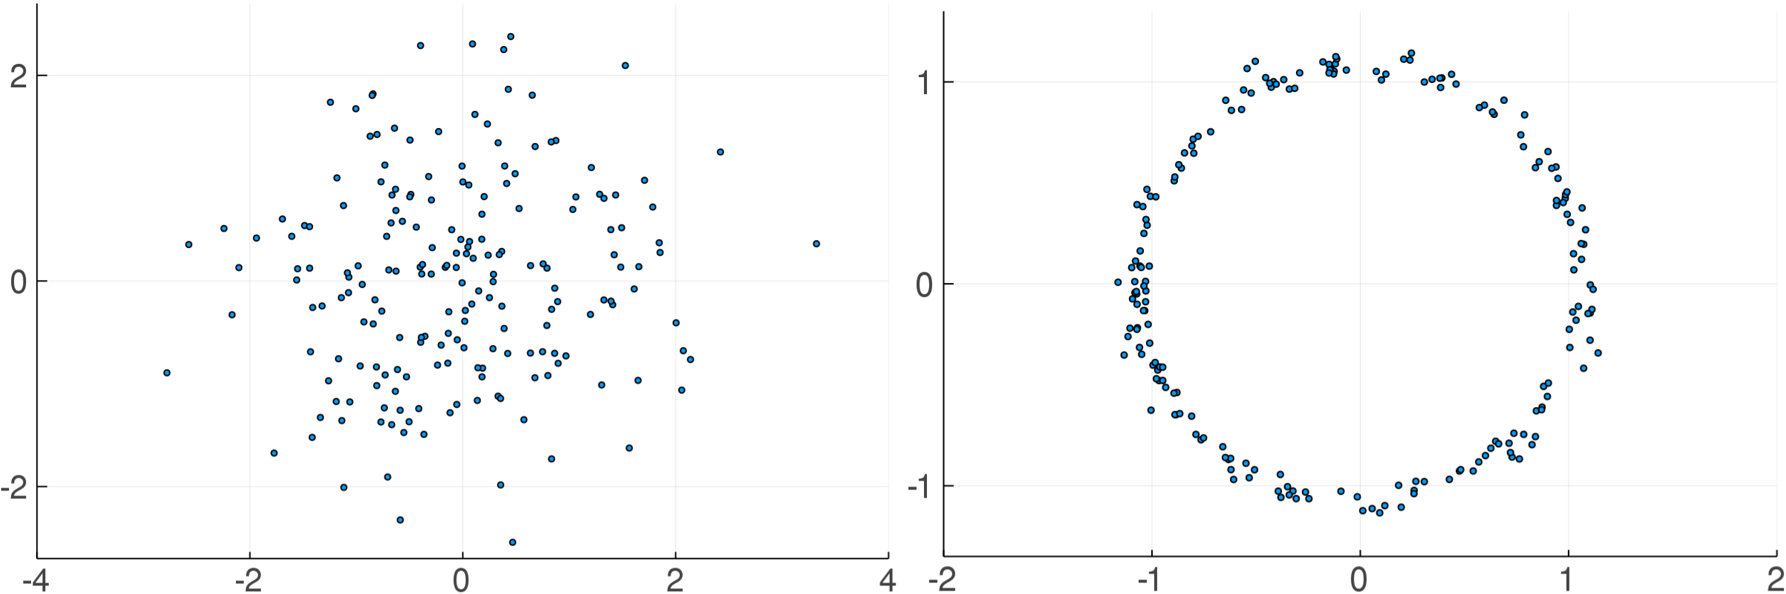
\includegraphics[scale=0.4]{normalverteilt}
		\captionsetup{labelformat=empty}
		\caption{Gegeben die Realisierungen einer Zufallsvariablen $\z\sim \mathcal{N}(\mathbf{0},\mathbf{I})$  (Links) lässt sich mit Abbildung durch eine Funktion, hier $g(\textbf{z})= \frac{\textbf{z}}{15}+\frac{\textbf{z}}{||\textbf{z}||}$ eine ganz andere Verteilung erzeugen (Rechts). Dies nutzt der VAE aus, um aus Realisierungen einer normalverteilten Zufallsvariablen komplexe Verteilungen in großer Dimension zu modellieren. Die Funktion g, beim VAE der Decoder wird aus den Daten erlernt. \textbf{}\cite{tutvae}}
	\end{figure}

	Welche Verteilung für den Decoder $\pdec$ dafür am besten geeignet ist, hängt vom Typ der zu erzeugenden Daten ab.\\ Für binäre Daten  $\textbf{x}_{i} \in \{0,1\}^{D}$ werden wir eine multivariate Bernoulliverteilung verwenden, also $p_{\theta}(\textbf{x}_{i}|\textbf{z}) =  \mathcal{B}(\boldsymbol{p}_{i})$. Gemeint ist hiermit eine elementweise Auswertung univariater Bernoulliverteilungen.\\
	Für stetige Daten $\textbf{x}_{i} \in \mathbb{R}^{D}$ wählen wir eine multivariate Normalverteilung $p_{\theta}(\textbf{x}_{i}|\textbf{z}) = \mathcal{N}(\boldsymbol{\hat{\mu}}_{i},\boldsymbol{\hat{\sigma}}_{i}^{2}\textbf{I})$.\\
	Hierbei sind $\boldsymbol{\hat{\mu}}_{i} = \boldsymbol{\hat{\mu}}_{\boldsymbol\theta}(\textbf{z})$ und $\boldsymbol{\hat{\sigma}}_{i}^{2} = \boldsymbol{\hat{\sigma}}_{\boldsymbol\theta}^{2}(\textbf{z}) $ bzw. $\textbf{p}_{i} = \textbf{p}_{\boldsymbol\theta}(\textbf{z})$ die Ausgaben des Decodernetzwerkes.\newpage
	\begin{figure}[h!]
		\centering
		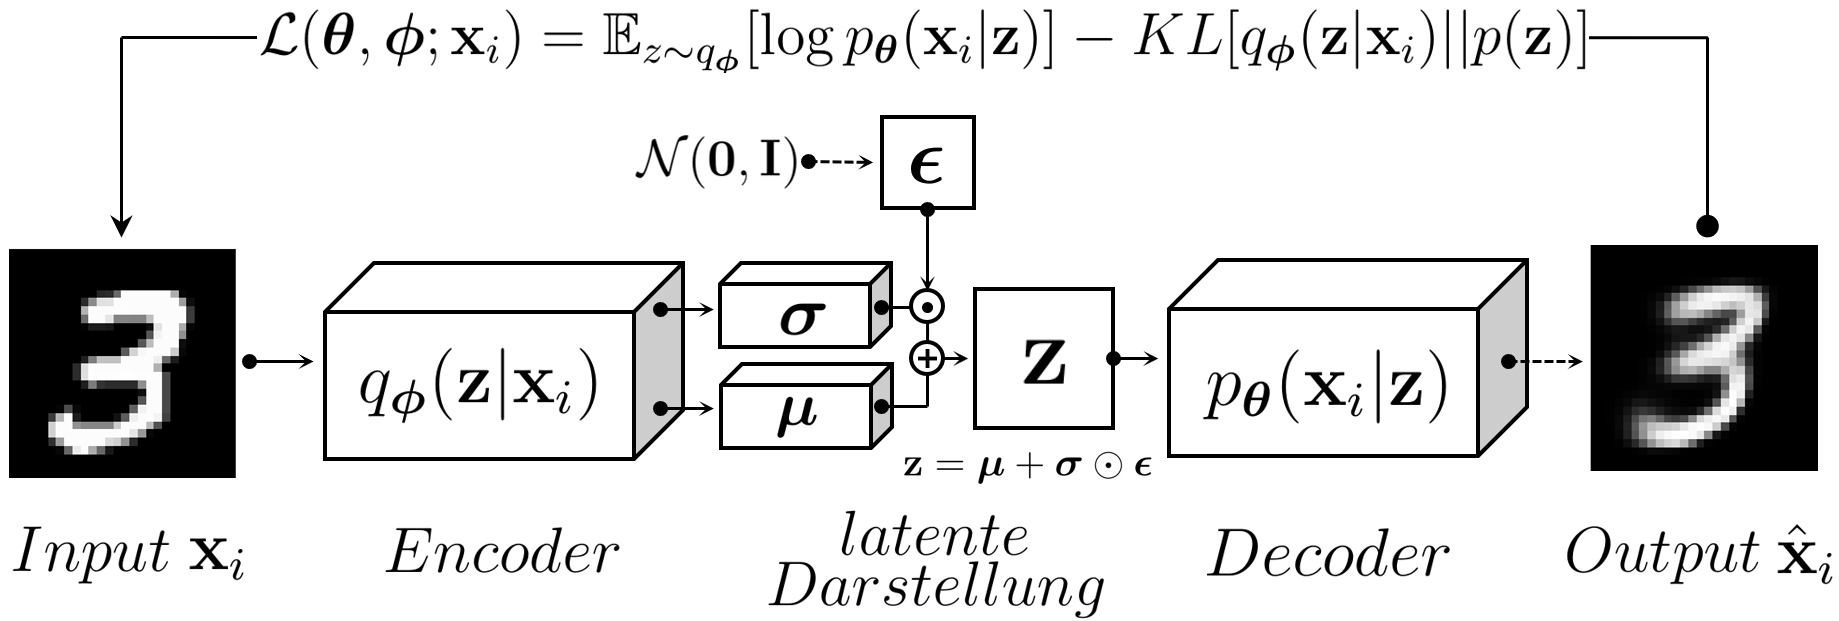
\includegraphics[scale=0.41]{VAE-Modell}
		\captionsetup{labelformat=empty}
		\caption{Schematische Darstellung eines Variational Autoencoders. Der hochdimensionale Input $\mathbf{x}_i$ wird durch den Encoder auf einen Erwartungswertvektor $\boldsymbol{\mu}$ und Streuungsparameter $\boldsymbol{\sigma}$ abgebildet. Anschließend wird eine niedrigdimensionale latente Darstellung \textbf{z} gezogen. Dabei wird der Reparametrisierungstrick $\textbf{z}=\boldsymbol{\mu}+\boldsymbol{\sigma} \odot \boldsymbol{\epsilon}$ angewandt. Der Decoder rekonstruiert nun mit dieser Darstellung einen Output $\hat{\mathbf{x}}_i$. Der Modellverlust ist durch die negative ELBO gegeben, durch Minimierung dieser kann das Modell optimiert werden.\\}
		\centering
		\begin{minipage}{.5\textwidth}
			\centering
			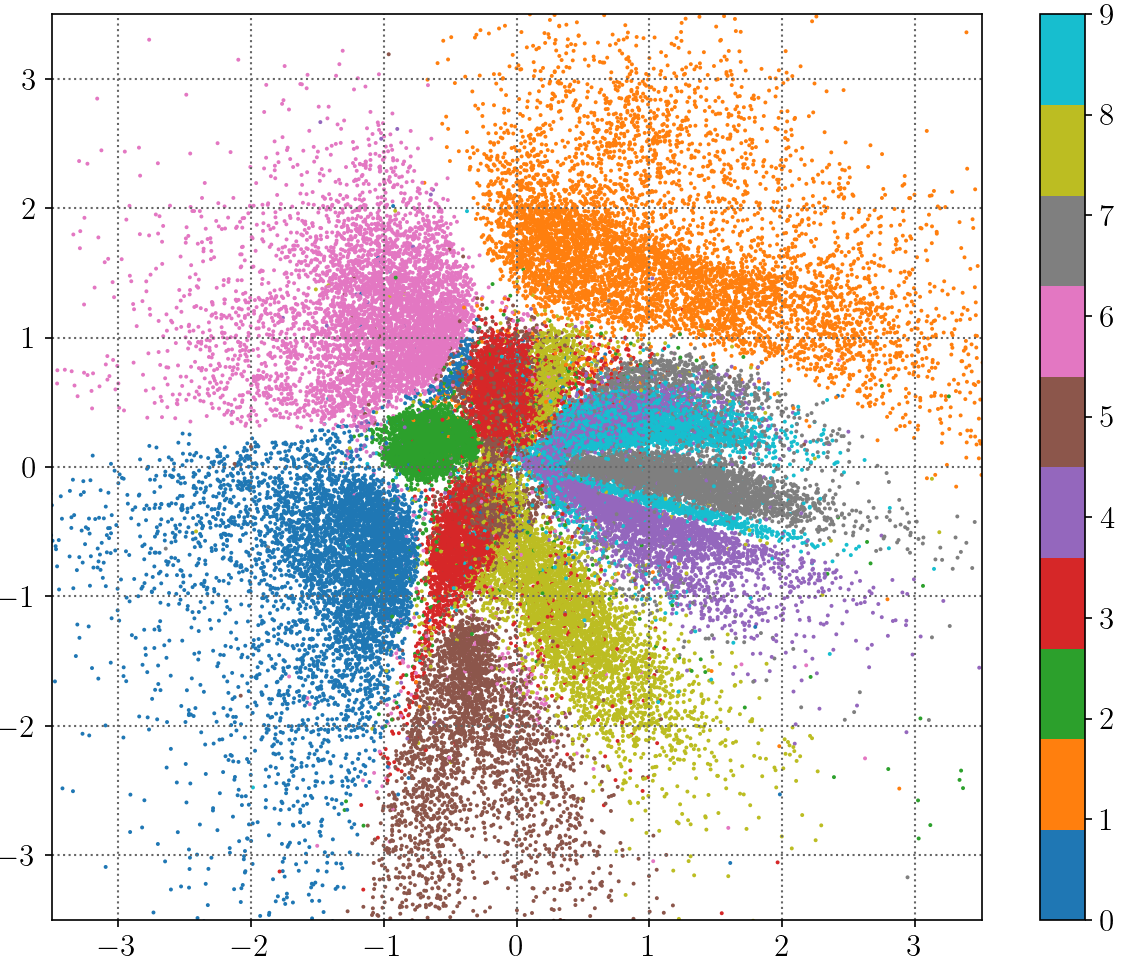
\includegraphics[scale=0.43]{latent_space_2D}
		\end{minipage}%
		\begin{minipage}{.5\textwidth}
			\centering
			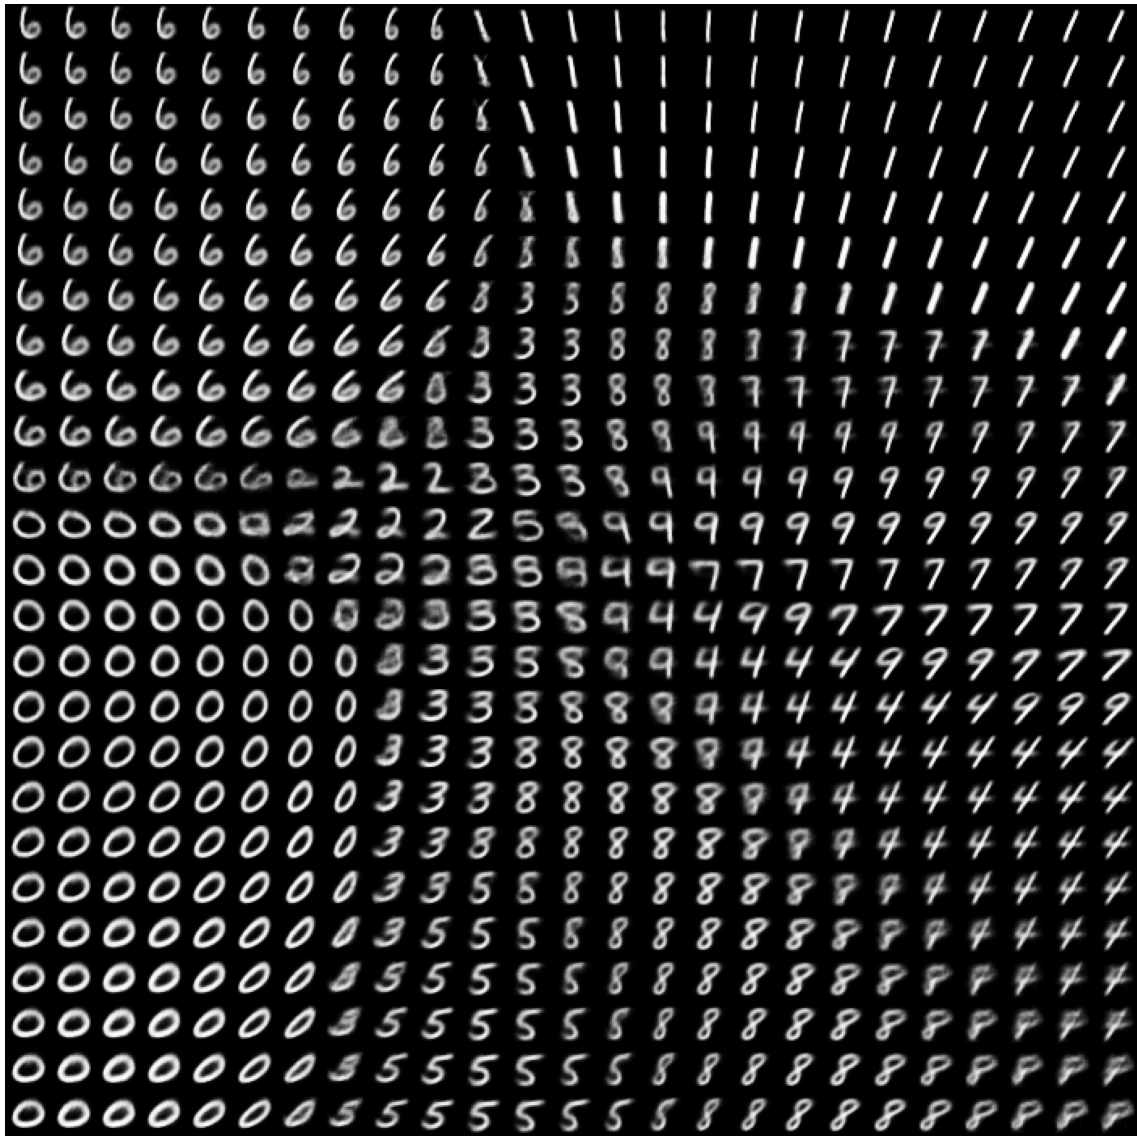
\includegraphics[scale=0.36]{latent_space_2D_reconstructions}
		\end{minipage}
		\captionsetup{labelformat=empty}
		\caption{Erlernte latente Darstellung des MNIST-Trainingsdatensatzes im zweidimensionalen\\ latenten Raum (links) und durch das Decodernetzwerk erzeugte Daten. (rechts) Die \\latenten Darstellungen $\mathbf{z}$ wurden mit linearem Abstand im Quadrat $[-2,2]^2$ gewählt. Auf die verwendete Modellstruktur und den dazu geschriebenen Code gehen wir im praktischen Teil dieser Arbeit genauer ein. }
	\end{figure}
	Für eine konkrete Berechnung der ELBO betrachten wir zuerst die KL-Divergenz der nun parameterfreien Verteilung $p(\textbf{z})$ nach $q_{\boldsymbol\phi}(\textbf{z}|\textbf{x}_{i})$. $d$ notiert hierbei die Dimension der latenten Darstellung und $p_{\mathcal{N}(\boldsymbol\mu_{i},\boldsymbol\sigma_{i}^{2}\mathbf{I})}(\textbf{z})$ bzw. $p_{\mathcal{N}(\mathbf{0},\mathbf{I})}(\textbf{z})$ die Auswertung der jeweiligen Dichtefunktion an der Stelle $\textbf{z}$.

	\begin{align*}
	D_{KL}\big(q_{\boldsymbol\phi}(\textbf{z}|\textbf{x}_{i}) || p(\textbf{z})\big) &= \mathbb{E}_{\z\sim\mathcal{N}(\boldsymbol\mu_{i},\boldsymbol\sigma_{i}^{2}\mathbf{I})}\left[\log\left(\frac{p_{\mathcal{N}(\boldsymbol\mu_{i},\boldsymbol\sigma_{i}^{2}\mathbf{I})}(\textbf{z})}{p_{\mathcal{N}(\mathbf{0},\mathbf{I})}(\textbf{z})}\right)\right].\\
	&= \mathbb{E}_{\z\sim\mathcal{N}(\boldsymbol\mu_{i},\boldsymbol\sigma_{i}^{2}\mathbf{I})}\big[\log\big(p_{\mathcal{N}(\boldsymbol\mu_{i},\boldsymbol\sigma_{i}^{2}\mathbf{I})}(\textbf{z})\big)
	- \log\big(p_{\mathcal{N}(\mathbf{0},\mathbf{I})}(\textbf{z})\big)\big].
	\end{align*}
	Die jeweiligen Dichtefunktionen sind durch
	\begin{align*}
	p_{\mathcal{N}(\boldsymbol\mu_{i},\boldsymbol\sigma_{i}^{2}\mathbf{I})}(\textbf{z})&= \frac{1}{\sqrt{2\pi^{d} \det(\boldsymbol\sigma_{i}^{2}\mathbf{I})}}\exp\left(-\frac{1}{2}(\textbf{z}-\boldsymbol\mu_{i})^{\mathrm{T}}(\boldsymbol\sigma_{i}^{2}\mathbf{I})^{-1}(\textbf{z}-\boldsymbol\mu_{i})\right) \notag \\
	\log(p_{\mathcal{N}(\boldsymbol\mu_{i},\boldsymbol\sigma_{i}^{2}\mathbf{I})}(\textbf{z}))&= -\frac{1}{2}\big(\log(2\pi^{d} \det(\boldsymbol\sigma_{i}^{2}\mathbf{I}))+(\textbf{z}-\boldsymbol\mu_{i})^{\mathrm{T}}(\boldsymbol\sigma_{i}^{2}\mathbf{I})^{-1}(\textbf{z}-\boldsymbol\mu_{i})\big)\\ \notag
	\log(p_{\mathcal{N}(\mathbf{0},\mathbf{I})}(\textbf{z}))&= -\frac{1}{2}\left(\log(2\pi^{d} )+\textbf{z}^{\mathrm{T}}\mathbf{I}\textbf{z}\right)
	\end{align*}
	gegeben. Einsetzen und aufteilen des Erwartungswertes liefert uns
	\begin{align*}
	&\mathbb{E}_{\z\sim\mathcal{N}(\boldsymbol\mu_{i},\boldsymbol\sigma_{i}^{2}\mathbf{I})}\Big[-\frac{1}{2}\Big(\log\big(\det(\boldsymbol\sigma_{i}^{2}\mathbf{I})\big)+(\textbf{z}-\boldsymbol\mu_{i})^{\mathrm{T}}(\boldsymbol\sigma_{i}^{2}\mathbf{I})^{-1}(\textbf{z}-\boldsymbol\mu_{i})-\textbf{z}^{\mathrm{T}}\mathbf{I}\textbf{z}\Big)\Big]\\
	=
	&-\frac{1}{2}\Big(\log\big(\det(\boldsymbol\sigma_{i}^{2}\mathbf{I})\big)+\mathbb{E}_{\z\sim\mathcal{N}(\boldsymbol\mu_{i},\boldsymbol\sigma_{i}^{2}\mathbf{I})}\big[(\textbf{z}-\boldsymbol\mu_{i})^{\mathrm{T}}(\boldsymbol\sigma_{i}^{2}\mathbf{I})^{-1}(\textbf{z}-\boldsymbol\mu_{i})\big]-\mathbb{E}_{\z\sim\mathcal{N}(\boldsymbol\mu_{i},\boldsymbol\sigma_{i}^{2}\mathbf{I})}\big[\textbf{z}^{\mathrm{T}}\mathbf{I}\textbf{z}\big]\Big).
	\end{align*}
	Da $\z\sim\mathcal{N}(\boldsymbol\mu_{i},\boldsymbol\sigma_{i}^{2})$ gilt für die Quadratischen Formen \cite{matrix}:
	\begin{align*}
	\mathbb{E}_{\z\sim\mathcal{N}(\boldsymbol\mu_{i},\boldsymbol\sigma_{i}^{2}\mathbf{I})}\big[\textbf{z}^{\mathrm{T}}\mathbf{I}\textbf{z}\big] &= \boldsymbol\mu_{i}^{\mathrm{T}}\mathbf{I}\boldsymbol\mu_{i}+\mathrm{Tr}(\boldsymbol\sigma_{i}^{2}\mathbf{I})\\ \mathbb{E}_{\z\sim\mathcal{N}(\boldsymbol\mu_{i},\boldsymbol\sigma_{i}^{2}\mathbf{I})}\big[(\textbf{z}-\boldsymbol\mu_{i})^{\mathrm{T}}(\boldsymbol\sigma_{i}^{2}\mathbf{I})^{-1}(\textbf{z}-\boldsymbol\mu_{i})\big] &= \mathrm{Tr}((\boldsymbol\sigma_{i}^{2}\mathbf{I})^{-1}\boldsymbol\sigma_{i}^{2}\mathbf{I}).
	\end{align*}


	Nun lässt sich mit ${\boldsymbol\sigma_{i}^{2}\mathbf{I}} =  \begin{psmallmatrix}\sigma_{i,1}^{2} & \ &\ \\ \ & \ddots &\ \\ \ & \ &\sigma_{i,d}^{2}\end{psmallmatrix}$ die KL-Divergenz ausrechnen.
	\begin{align*}
	&-\frac{1}{2}\Big(\log\big(\det(\boldsymbol\sigma_{i}^{2}\mathbf{I})\big)+\mathrm{Tr}((\boldsymbol\sigma_{i}^{2}\mathbf{I})^{-1}\boldsymbol\sigma_{i}^{2}\mathbf{I})-\boldsymbol\mu_{i}^{\mathrm{T}}\textbf{I}\boldsymbol\mu_{i}-\mathrm{Tr}(\boldsymbol\sigma_{i}^{2}\mathbf{I})\Big) \notag \\
	= &-\frac{1}{2}\left(\log\Big(\prod_{j=1}^{d}\sigma_{i,j}^{2}\Big)+d-\sum_{j=1}^{d}\mu_{i,j}^{2}-\sum_{j=1}^{d}\sigma_{i,j}^{2}\right) \notag \\
	= &-\frac{1}{2}\sum_{j=1}^{d}\Big(\log\big(\sigma_{i,j}^{2}\big)+1-\mu_{i,j}^{2}-\sigma_{i,j}^{2}\Big).
	\end{align*}

	Auch $\pdec$ kann mit unserer Wahl der Verteilungen explizit ausgerechnet werden.
	Mit $D$ wird dazu die Dimension des Inputs und Outputs notiert.
	Für die Verwendung einer multivariaten Normalverteilung im Decoder ergibt sich:
	\begin{align*}
	\log\big(\pdec)\big) &=  \log\big(p_{\mathcal{N}(\boldsymbol{\hat{\mu}}_{i},\boldsymbol{\hat{\sigma}}_{i}^{2}\textbf{I})}(\textbf{x}_{i})\big)\notag \\
	&= -\frac{1}{2}\left(\log(2\pi^{D} \det(\boldsymbol{\hat{\sigma}}_{i}^{2}\textbf{I}))+(\textbf{x}_{i}-\boldsymbol{\hat{\mu}}_{i})^{\mathrm{T}}(\boldsymbol{\hat{\sigma}}_{i}^{2}\textbf{I})^{-1}(\textbf{x}_{i}-\boldsymbol{\hat{\mu}}_{i})\right) \notag \\
	&= -\frac{1}{2}\left(\log(2\pi^{D})+\log\Big( \prod_{p=1}^{D}\hat{\sigma}_{i,p}^{2}\Big)+  \begin{pmatrix}  \frac{x_{i,1}-\hat{\mu}_{i,1}}{\hat{\sigma}_{i,1}^{2}}&\cdots& \frac{x_{i,D}-\hat{\mu}_{i,D}}{\hat{\sigma}_{i,D}^{2}}\end{pmatrix}
	\boldsymbol{\cdot}(\textbf{x}_{i}-\boldsymbol{\hat{\mu}}_{i})\right) \notag \\
	&= -\frac{1}{2}\left(D\log(2\pi)+\sum_{p=1}^{D}\log\left( \hat{\sigma}_{i,p}^{2}\right)+
	\sum_{p=1}^{D}\frac{\big(x_{i,p}-\hat{\mu}_{i,p}\big)^{2}}{\hat{\sigma}_{i,p}^{2}}\right) \notag \\
	&= -\frac{1}{2}\sum_{p=1}^{D} \left(\log\left(2\pi \hat{\sigma}_{i,p}^{2}\right) + \frac{\big(x_{i,p}-\hat{\mu}_{i,p}\big)^{2}}{\hat{\sigma}_{i,p}^{2}}\right)
	\end{align*}

	Für eine bernoulliverteilte Zufallsvariable ist die Dichtefunktion  durch $p_{\mathcal{B}(\mathrm{p}_{i})}(x_{i}) = \mathrm{p}_{i}^{x_{i}}(1-\mathrm{p}_{i})^{(1-x_{i})}$ definiert. Somit ergibt sich für die Verwendung der multivariaten Bernoulliverteilung im Decoder: \\
	\begin{align*}
	\log\big(p_{\theta}(\textbf{x}_{i}|\textbf{z})\big) &=  \log\big(p_{\mathcal{B}(\boldsymbol{p}_{i})}(\textbf{x}_{i})\big)\notag \\
	&= \log\left(p_{\mathcal{B}(\mathrm{p}_{1})}\left(x_{i,1}\right)\ \cdot\ldots\cdot \ p_{\mathcal{B}(\mathrm{p}_{D})}\left(x_{i,D}\right)\right)\notag \\
	&= \log\left(\prod_{p=1}^{D}\left(p_{i,p}\right)^{x_{i,p}}\left(1-p_{i,p}\right)^{\left(1-x_{i,p}\right)}\right) \notag \\
	&=  \sum_{p=1}^{D}x_{i,p}\log\left(p_{i,p}\right)+\left(1-x_{i,p}\right)\log\left(1-p_{i,p}\right)
	\end{align*}
	\subsection[ODE$^2$VAE]{Second Order ODE-Variational Autoencoder}
	Gegeben sei eine \emph{time series} $\mathbf{x}_{0:T}=(\mathbf x_{0}, \mathbf x_{1}, \ldots,\mathbf x_{T})\in \mathbb{R}^{D\times T}$ zu observierten Zeitpunkten $t_{0}, t_{1},\ldots,t_{T}$ mit zugehörigen latenten Zuständen $\mathbf z_{0:T}=(\mathbf z_{0}, \mathbf z_{1}, \ldots, \mathbf z_{T})\in \mathbb{R}^{d\times T}$ geringerer Dimension. \\
	Wir nehmen an, dass die zeitliche Änderung der latenten Zustände durch eine Differentialgleichung beschrieben werden kann. Das Vektorfeld der Differentialgleichung wird durch ein Neuronales Netzwerk $f_{\boldsymbol{\psi}}$, ein \emph{ODE-Network} in stetiger Zeit $t$ modelliert.
	\begin{align*}
	\dfrac{\partial \mathbf{z}(t)}{\partial t}&=f_{\boldsymbol{\psi}}(\mathbf{z}(t),t), \\
	\mathbf z(t_{0})&=\mathbf z_{0}
	\end{align*}
	Durch einen gegebenen Anfangswert $\mathbf z_{0}$ erhalten wir für lipschitzstetige Funktionen immer eine Lösung des Anfangswertproblems
	\begin{align*}
	\mathbf z_{T}=\mathbf z_{0} +\int_{0}^{T} f_{\boldsymbol{\psi}}(\mathbf{z}(t),t) \mathrm{d}t.
	\end{align*}
	Das Integral lässt sich numerisch mit ODE-Solvern berechnen. \\
	Wir benutzen einen VAE zur Dimensionsreduzierung. Der Encoder bestimmt den Anfangswert $\mathbf z_{0}$ der Differentialgleichung, welcher mit dem ODE-Netzwerk eine eindeutig bestimmte Kurve im latenten Raum liefert. Der Decoder rekonstruiert anschließend zu den Zeitpunkten $t_{0}, t_{1},\ldots,t_{T}$ die Inputsequenz $\mathbf x_{0:T}$. \\ \\
	ODEs erster Ordnung sind jedoch nicht in der Lage Datensätze zufriedenstellend zu modellieren, bei denen sich auch höhere Momente ändern.
	Wir werden daher ODEs zweiter Ordnung verwenden, welche sich äquivalent als ein System bestehend aus zwei Differenti\nolinebreak algleichungen erster Ordung notieren lassen.\\ Der Zustand $\mathbf z_{t}=(\mathbf s_{t}, \mathbf v_{t})^{\mathrm{T}}$ zum Zeitpunkt $t$, wird dazu in eine Positionskomponente $\mathbf s_{t}$ und eine Geschwindigkeitskomponente $\mathbf v_{t}$ zerlegt, deren Anfangswerte $\mathbf s_{0}$ und $\mathbf v_{0}$ von zwei unterschiedlichen Encoder-Netzwerken, dem \emph{Position-Encoder} und dem \emph{Velocity-Encoder}, erlernt werden.\\
	Der Position-Encoder erhält zur Bestimmung der latenten Positionskomponente die erste Komponente $\mathbf x_{0}$ der Inputsequenz, während der Velocity-Encoder die ersten $m\geq 3$ Komponenten $\mathbf x_{0:m}$ der Inputsequenz erhällt. Dies ermöglicht uns das Encodieren der höheren Momente.
	\begin{align*}
	\dfrac{\partial^2 \mathbf{z}(t)}{\partial^2 t}&=f_{\boldsymbol{\psi}}\left(\mathbf{z}(t), \tfrac{\partial \mathbf{z}(t)}{\partial t}, t\right), \\
	\begin{cases*}
	\tfrac{\partial \mathbf{s}(t)}{\partial t}=\mathbf v(t) \\
	\tfrac{\partial \mathbf{v}(t)}{\partial t}=f_{\boldsymbol{\psi}}(\mathbf s(t), \mathbf v(t), t) \\
	\end{cases*},
	\left(\begin{array}{cc}
	\mathbf s_{T} \\
	\mathbf v_{T}
	\end{array}\right)
	&=
	\left(\begin{array}{cc}
	\mathbf s_{0} \\
	\mathbf v_{0}
	\end{array}\right)
	+
	\int_{0}^{T}
	\left(\begin{array}{cc}
	\mathbf v(t) \\
	f_{\boldsymbol{\psi}}(\mathbf s(t), \mathbf v(t), t)
	\end{array}\right)
	\mathrm{d}t.
	\end{align*}
	Die Autoren des Papers verwenden ein Bayensisches Neuronales Netzwerk zur Modellierung der Differentialgleichung um Unsicherheit besser darstellen zu können. Wir werden aber auf ein gewöhnliches Neuronales Netzwerk zurückgreifen und im nächsten Kapitel auf die Modellierung Stochastischer Differentialgleichung eingehen.
	\begin{figure}[h!]
		\centering
		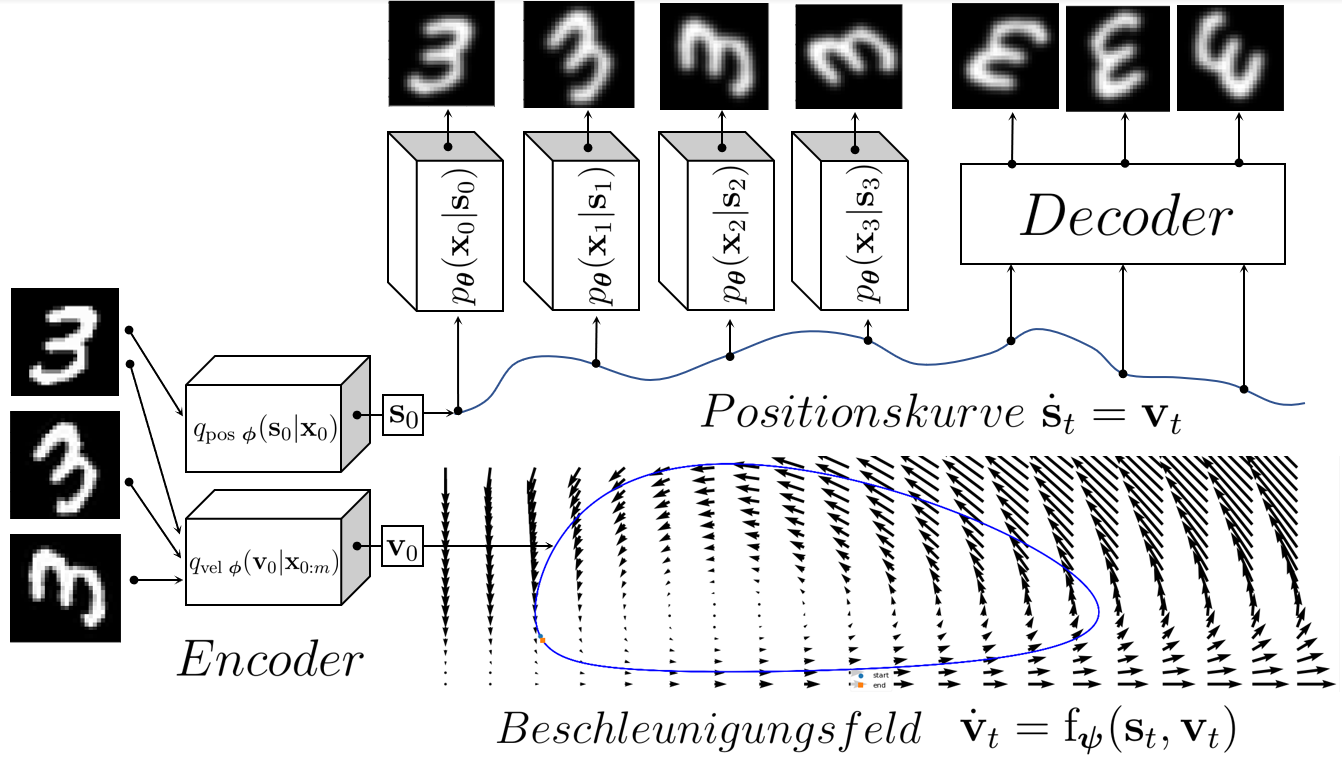
\includegraphics[scale=0.57]{ODE2VAE_ODE_Net}
		\captionsetup{labelformat=empty}
		\caption{Schematische Darstellung des ODE$^2$VAE. Eine Inputsequenz wird von den Encodermodellen auf die Startwerte einer Beschleunigungs- und Positionskurve abgebildet. Die Änderung der Geschwindigkeitskurve (blau) wird durch ein ODE-Net modelliert und mit einem ODEsolver berechnet. Die Änderung der Positionskurve ergibt sich durch Integrati\nolinebreak on über die Geschwindigkeitskurve. Zu festgelegten Zeitpunkten rekonstruiert der Decoder aus den Positionswerten $\mathbf{s}_t$ die Inputsequenz.}
	\end{figure}

	Als Trainingskriterium des ODE$^2$VAE verwenden wir erneut die negative ELBO.
	Wir erhalten:
	\begin{align*}
	\log\big(p_{\boldsymbol{\theta}}(\mathbf{x}_{0:T})\big)&\ge \E_{\mathbf{z}_{0:T}\sim q_{\boldsymbol\phi,\boldsymbol\psi}}
	\left[\log\big(p_{\boldsymbol\theta}\left(\mathbf{x}_{0:T}|\mathbf{z}_{0:T}\right)\big)\right] - D_{KL}\big[q_{\boldsymbol\phi,\boldsymbol\psi}(\mathbf{z}_{0:T}|\mathbf{x}_{0:m})||p_{\boldsymbol\theta,\boldsymbol\psi}(\mathbf{z}_{0:T})\big]\\
	&=\underbrace{\E_{\mathbf{z}_{0}\sim q_{\text{enc }\boldsymbol\phi}}
		\left[\log\big(p_{\boldsymbol\theta}\left(\mathbf{x}_{0}|\mathbf{z}_{0}\right)\big)\right] - D_{KL}\big[q_{\text{enc }\boldsymbol\phi}(\mathbf{z}_{0}|\mathbf{x}_{0:m})||p_{\boldsymbol\theta}(\mathbf{z}_{0})\big]}_{\text{Vanilla-VAE ELBO}}\\ &+ \underbrace{\sum_{t=1}^T \E_{\mathbf{z}_{t}\sim q_{\text{ode }\boldsymbol\psi}}
		\left[\log\big(p_{\boldsymbol\theta}\left(\mathbf{x}_{t}|\mathbf{z}_{t}\right)\big)\right] - D_{KL}\big[q_{\text{ode }\boldsymbol\psi}(\mathbf{z}_{t}|\mathbf{x}_{0:m})||p_{\boldsymbol\theta,\boldsymbol\psi}(\mathbf{z}_{t})\big]}_{\text{Dynamischer Loss}}
	\end{align*}
	Der erste Teil ist die ELBO eines Standard-VAE's. \textbf{TODO für was steht der zweite Teil der ELBO}
	Als dem latenten Raum zugrundeliegenden Verteilung $p_{\boldsymbol\theta}(\mathbf{z}_{0})$ wählen wir eine parameterfreie Standardnormalverteilung $\mathcal{N}(\mathbf{0},\mathbf{I})$.\\
	Die Encoder-Verteilung ist als Normalverteilung mit $\mathbf{z}_{0} = (\mathbf{s}_{0},\mathbf{v}_{0})^{\mathrm{T}}$ durch
	\begin{align*}
	q_{\text{enc }\boldsymbol\phi}(\mathbf{z}_{0}|\mathbf{x}_{0:m}) =
	\mathcal{N}\left(\left(\begin{array}{cc}
	\boldsymbol\mu_{\text{pos }\boldsymbol\phi}(\textbf{x}_{0}) \\
	\boldsymbol\mu_{\text{vel }\boldsymbol\phi}(\textbf{x}_{0:m})
	\end{array}\right),\left(\begin{array}{cc}
	\text{diag}(\boldsymbol\sigma_{\text{pos }\boldsymbol\phi}(\textbf{x}_{0})) &
	\mathbf{0}\\
	\mathbf{0} &
	\text{diag}(\boldsymbol\sigma_{\text{vel }\boldsymbol\phi}(\textbf{x}_{0:m}))
	\end{array}\right)\right)
	\end{align*}
	gegeben. Wie erläutert hängt der Output des Velocity-Encoders dabei von den ersten $m\ge3$ Zuständen ab, während der Output des Position-Encoders nur durch den ersten Zustand bestimmt wird.\\
	Die Berechnung des \emph{reconstruction loss} ist von der Wahl der im Decoder verwendeten Verteilung abhängig. Für unsere Datensätze werden wir eine Bernoulliverteilung verwenden.
	Die analytische Berechnung ist nun mit den Resultaten des letzten Kapitels möglich.\\
	Die Berechnung des \emph{dynamic loss} ist komplizierter. \\
	Der \emph{reconstruction loss} $\E_{\mathbf{z}_{t}\sim q_{\text{ode }\boldsymbol\psi}}
	\left[\log\big(p_{\boldsymbol\theta}\left(\mathbf{x}_{t}|\mathbf{z}_{t}\right)\big)\right] $ lässt sich zwar mit den Resultaten des ersten Kapitels berechnen, für die approximative Berechnung der KL-Divergenz
	\begin{align*}
	D_{KL}\big[q_{\text{ode }\boldsymbol\psi}(\mathbf{z}_{t}|\mathbf{x}_{0:m})||p_{\boldsymbol\theta,\boldsymbol\psi}(\mathbf{z}_{t})\big]
	&=\mathbb{E}_{\mathbf{z}_{t}\sim q_{\text{ode }\boldsymbol\psi}}\big[\log\big(q_{\text{ode }\boldsymbol\psi}(\mathbf{z}_{t}|\mathbf{x}_{0:m}) \big) - \log\big(p_{\boldsymbol\theta,\boldsymbol\psi}(\mathbf{z}_{t}) \big)\big] \\
	\overset{\text{M.C.}}&{\simeq} \frac{1}{L} \sum_{i=1}^{L} \log\big(q_{\text{ode }\boldsymbol\psi}(\mathbf{z}_{t}|\mathbf{x}_{0:m}) \big) - \log\big(p_{\boldsymbol\theta,\boldsymbol\psi}(\mathbf{z}_{t}) \big)
	\end{align*}
	%eventuell noch darauf eingehen, warum q_ode eine Verteilung ist.
	benötigen wir jedoch die log-Dichten der ODE-Verteilung $q_{\text{ode }\boldsymbol\psi}(\mathbf{z}_{t}|\mathbf{x}_{0:m})$ und die der Prior-Verteilung $p_{\boldsymbol\theta,\boldsymbol\psi}(\mathbf{z}_{t})$.\\
	Die latenten Werte $\mathbf{z}_{t} = (\mathbf{s}_{t},\mathbf{v}_{t})^{\mathrm{T}}$ sind nun aber nicht mehr von den Encoder-Netzwerken abhängig, sondern werden durch die Neural-ODE $f_{\boldsymbol\psi}(\mathbf{s}_{t},\mathbf{v}_{t})$ bestimmt.
	Zur Berechnung der log-Dichte der ODE-Verteilung lassen sich folgende hilfreiche Theoreme anwenden.
	\begin{theorem}
		Sei $\mathbf{z}(t)$ eine stetige Zufallsvariable mit einer von der Zeit abhängigen Dichtefunktion $q(\mathbf{z}(t))$. Sei $\tfrac{\partial \mathbf{z}(t)}{\partial t}=f(\mathbf{z}(t),t)$ eine in $\mathbf{z}$ Lipschitzstetige und in $t$ stetige Differentialgleichung, welche die Veränderung von $\mathbf{z}(t)$ mit der Zeit beschreibt.
		Die Veränderung der Dichte folgt nun ebenfalls einer Differentialgleichung:
		\begin{align*}
		\dfrac{\partial \log\big(q(\mathbf{z}(t))\big)}{\partial t}&= - \mathrm{Tr}\left(\dfrac{\partial f}{\partial\mathbf{z}}(t)\right).
		\end{align*}
	\end{theorem}
	\begin{proof}
		Ein ausführlicher Beweis und weitere Erklärungen sind  in \emph{Neural Ordinary Differential Equations} \cite{neuralode} zu finden.
	\end{proof}
	Die Berechnung der Spur der Jacobimatrix unserer Differentialgleichung $f_{\boldsymbol\psi}(\mathbf{s}_{t},\mathbf{v}_{t})$ erfordert entsprechend der gewählten latenten Dimension $d$ auch eine $d$-fache Auswertung des zugrundeliegenden Netzwerkes. Um den Rechenaufwand deutlich zu verringern, verwenden wir zwei Tricks.\cite{ffjord}\\
	Das Vektor-Matrix Produkt $\boldsymbol\epsilon^\mathrm{T} \cdot \tfrac{\partial f}{\partial\mathbf{z}}(t)$ lässt sich durch \emph{Reverse-Mode Automatic Differentiation} mit einmaliger Auswertung der Funktion $f$ berechnen und die Spur einer Matrix kann durch ein doppeltes Matrix-Vektorprodukt mit einem Zufallsvektor $\boldsymbol\epsilon$ erwartungstreu geschätzt werden.

	\begin{theorem}%{$\mathrm{(Hutchinsons\ Spur\ Schätzer)}$}
		Sei $\mathbf{M}\in \mathbb{R}^{d \times d}$ eine beliebige Matrix und $\boldsymbol\epsilon \sim p(\boldsymbol\epsilon)$ eine Zufallsvariable mit $\E[\boldsymbol\epsilon] = \mathbf{0}$ und $\mathrm{Cov}(\boldsymbol\epsilon) =\mathbf{I}$. Die Spur der Matrix $\mathbf{M}$ lässt sich erwartungstreu durch ein doppeltes Matrix-Vektorprodukt der Matrix  $\mathbf{M}$ mit dem Zufallvektor $\boldsymbol\epsilon$ schätzen:
		\begin{align*}
		\mathrm{Tr}(\mathbf{M}) =
		\E_{\boldsymbol\epsilon \sim p(\boldsymbol\epsilon)}\big[\boldsymbol\epsilon^\mathrm{T} \mathbf{M} \boldsymbol\epsilon \big].
		\end{align*}
	\end{theorem}
	\begin{proof} Wir orientieren uns an \cite{Hutchin}.
		Für $\boldsymbol\epsilon \sim p(\boldsymbol\epsilon)$ mit $\E[\boldsymbol\epsilon] = \mathbf{0}$ und $\mathrm{Cov}(\boldsymbol\epsilon) =\mathbf{I}$ gilt $\E_{\boldsymbol\epsilon\sim p(\boldsymbol\epsilon)}[\boldsymbol\epsilon^\mathrm{T}\boldsymbol\epsilon] = \mathbf{I}.$ Wir erhalten nun für die Spur einer Matrix $\mathbf{M}$:
		\begin{align*}
		\mathrm{Tr}(\mathbf{M}) = \mathrm{Tr}(\mathbf{MI}) = \mathrm{Tr}(\mathbf{M\E_{\boldsymbol\epsilon\sim p(\boldsymbol\epsilon)}[\boldsymbol\epsilon^\mathrm{T}\boldsymbol\epsilon]}) = \E_{\boldsymbol\epsilon\sim p(\boldsymbol\epsilon)}[\mathrm{Tr}(\mathbf{M}\boldsymbol\epsilon^\mathrm{T}\boldsymbol\epsilon)] =
		\E_{\boldsymbol\epsilon \sim p(\boldsymbol\epsilon)}\big[\boldsymbol\epsilon^\mathrm{T} \mathbf{M} \boldsymbol\epsilon \big].
		\end{align*}
	\end{proof}
	Wir werden $p(\boldsymbol\epsilon)$ als multivariate Standardnormalverteilung festlegen.\\
	Auch hier erlaubt uns eine groß gewählte Batchsize, z.B. $M\ge100$ die Anzahl der Ziehungen für Monte-Carlo Schätzung als $L=1$ zu wählen.\\
	\\
	Mit diesen Resultaten können wir die log-Dichte der ODE-Verteilung mit relativ geringem Rechenaufwand berechnen.
	Wir erhalten für die Veränderung dieser:
	\begin{align*}
	\dfrac{\partial \log\big(q_{\text{ode }\boldsymbol\psi}(\mathbf{z}_{t}|\mathbf{x}_{0:m})\big)}{\partial t}\overset{\text{T.1}}&{=} - \text{Tr}\left(\dfrac{\partial f_{\boldsymbol\psi}(\mathbf{z}_{t})}{\partial\mathbf{z}_{t}}\right) \\ &=
	- \text{Tr} \left(\begin{array}{cc}
	\dfrac{\partial\mathbf{v}_{t}}{\partial\mathbf{s}_{t}} &
	\dfrac{\partial\mathbf{s}_{t}}{\partial\mathbf{v}_{t}}\\
	\dfrac{\partial f_{\boldsymbol\psi}(\mathbf{s}_{t},\mathbf{v}_{t})}{\partial\mathbf{s}_{t}} &
	\dfrac{\partial f_{\boldsymbol\psi}(\mathbf{s}_{t},\mathbf{v}_{t})}{\partial\mathbf{v}_{t}}
	\end{array}\right)\\
	&=
	-\text{Tr}\left(\dfrac{\partial f_{\boldsymbol\psi}(\mathbf{s}_{t},\mathbf{v}_{t})}{\partial\mathbf{v}_{t}}\right)\\
	\overset{\text{T.2}}&{=} -\E_{\boldsymbol\epsilon\sim\mathcal{N}(0,\text{I})}\left[\boldsymbol\epsilon^\mathrm{T}\dfrac{\partial f_{\boldsymbol\psi}(\mathbf{z}_{t})}{\partial\mathbf{v}_{t}}\boldsymbol\epsilon\right].
	\end{align*}
	Durch Integration ergibt sich nun
	\begin{align*}
	\log\big(q_{\text{ode }\boldsymbol\psi}(\mathbf{z}_{t}|\mathbf{x}_{0:m})\big)&=\log\big(q_{\text{enc }\boldsymbol\psi}(\mathbf{z}_{0}|\mathbf{x}_{0:m})\big)-\int_0^t \E_{\boldsymbol\epsilon\sim\mathcal{N}(0,\text{I})}\left[\boldsymbol\epsilon^\mathrm{T}\dfrac{\partial f_{\boldsymbol\psi}(\mathbf{s}_{t},\mathbf{v}_{t})}{\partial\mathbf{v}_{t}}\boldsymbol\epsilon\right]\text{d}t\\
	&= \log\big(q_{\text{enc }\boldsymbol\psi}(\mathbf{z}_{0}|\mathbf{x}_{0:m})\big)-\E_{\boldsymbol\epsilon\sim\mathcal{N}(0,\text{I})}\left[\int_0^t \boldsymbol\epsilon^\mathrm{T}\dfrac{\partial f_{\boldsymbol\psi}(\mathbf{s}_{t},\mathbf{v}_{t})}{\partial\mathbf{v}_{t}}\boldsymbol\epsilon\ \text{d}t\right]\\
	\overset{\text{M.C.}}&{\simeq} \log\big(q_{\text{enc }\boldsymbol\phi}(\mathbf{z}_{0}|\mathbf{x}_{0:m})\big)-\frac{1}{L}\sum_{i=1}^L\int_0^t \boldsymbol\epsilon^\mathrm{T}\dfrac{\partial f_{\boldsymbol\psi}(\mathbf{s}_{t},\mathbf{v}_{t})}{\partial\mathbf{v}_{t}}\boldsymbol\epsilon\ \text{d}t.
	\end{align*}
	Die Randbedingung $\log\big(q_{\text{enc }\boldsymbol\phi}(\mathbf{z}_{0}|\mathbf{x}_{0:m})\big)$ ist durch die Encoder-Verteilung gegeben.
	Der Erwartungswert wird durch Monte-Carlo Schätzung approximiert, $\boldsymbol\epsilon$ wird außerhalb des Integrals aus einer Standartnormalverteilung gezogen und das Integral numerisch durch ODE-Integratoren zusammen mit unserer Differentialgleichung berechnet.\\
	\begin{align*}
	\dfrac{\partial h(t)}{\partial t}&=\begin{cases*}
	\tfrac{\partial \mathbf{s}(t)}{\partial t}=\mathbf v(t) \\
	\tfrac{\partial \mathbf{v}(t)}{\partial t}=f_{\boldsymbol{\psi}}(\mathbf s(t), \mathbf v(t), t) \\
	\tfrac{\partial (\log\mathbf{q}(t))}{\partial t}= -\boldsymbol\epsilon^\mathrm{T}\tfrac{\partial f_{\boldsymbol\psi}(\mathbf{s},\mathbf{v},t)}{\partial\mathbf{v}}(t)\boldsymbol\epsilon
	\end{cases*}\\ h(t_T)&=\text{ODEintegrate}\big(h,h(t_0),t_1,t_2,\ldots,t_T,\boldsymbol\epsilon,f_{\boldsymbol\psi}\big)
	\end{align*}
	Der Wert
	$\log\big(p_{\boldsymbol\theta,\boldsymbol\psi}(\mathbf{z}_{t}) \big)$, der ebenfalls für die Berechnung der KL-Divergenz benötigt wird ist nicht bestimmbar. Müsste man doch die log-Dichten mit der unbekannten, "wahren"\  Funktion $f_{\boldsymbol\psi^{*}}(\mathbf{s}_{t},\mathbf{v}_{t})$ mit oben hergeleiteter Formel ausrechnen.
	Die Autoren des Papers treffen eine vereinfachende Annahme und legen wie bereits für den ersten Zustand geltend $p_{\boldsymbol\theta,\boldsymbol\psi}(\mathbf{z}_{t}) = \mathcal{N}(\mathbf{0},\mathbf{I})$ als parameterfreie multivariate Normalverteilung fest.\\
	Bei uns hat das aber zu dem Problem geführt, dass der KL-Term den \emph{reconstruction loss} stark übertrifft und das Verfahren im latenten Raum nur die Struktur einer Normalverteilung annehmen will ohne gleichzeitig den \emph{reconstruction loss} zufriedenstellend zu verringern. Wir greifen daher auf eine Abwandlung der im Paper vorgestellten alternativen Lossfunktion zurück. Das Verfahren konvergiert dann nur langsam und die Bilder neigen schnell dazu zu verschwimmen. \\
	\begin{align*}
	-\mathcal{L}(\boldsymbol\phi,\boldsymbol\psi,\boldsymbol\theta,\mathbf{x}_{0:T}) &=\underbrace{\E_{\mathbf{z}_{0}\sim q_{\text{enc }\boldsymbol\phi}}
		\left[\log\big(p_{\boldsymbol\theta}\left(\mathbf{x}_{0}|\mathbf{z}_{0}\right)\big)\right] - \gamma D_{KL}\big[q_{\text{enc }\boldsymbol\phi}(\mathbf{z}_{0}|\mathbf{x}_{0:m})||p_{\mathcal{N}(\mathbf{0},\mathbf{I})}(\z_0)\big]}_{\gamma\text{-VAE ELBO}}\\ &+ \underbrace{\sum_{t=1}^T \E_{\mathbf{z}_{t}\sim q_{\text{ode }\boldsymbol\psi}}
		\left[\log\big(p_{\boldsymbol\theta}\left(\mathbf{x}_{t}|\mathbf{z}_{t}\right)\big)\right] - \gamma D_{KL}\big[q_{\text{ode }\boldsymbol\psi}(\mathbf{z}_{t}|\mathbf{x}_{0:m})||p_{\mathcal{N}(\mathbf{0},\mathbf{I})}(\z_t)\big]}_{\text{Dynamischer Loss}} \\ &- \gamma \underbrace{\sum_{t=0}^{T-m} D_{KL}\big[q_{\text{ode }\boldsymbol\psi}(\mathbf{z}_{t}|\mathbf{x}_{0:m})||q_{\text{enc }\boldsymbol\phi}(\mathbf{z}_{t}|\mathbf{x}_{t:(t+m)})\big]}_{\text{KL-Divergenz zur Encoderverteilung}}
	\end{align*}
	Wir multiplizieren die KL-Divergenz mit einem Faktor $\gamma$, der im Verlauf des Trainings schrittweise von 0 auf 1 angehoben wird. So wird zu Beginn des Trainingsprozess das Anfertigen guter Rekonstruktionen priorisiert und die sinnvolle
	Anordnung der latenten Variablen im latenten Raum erst später im Trainingsprozess vorgenommen.\\
	Außerdem minimieren wir weiter die KL-Divergenz zur Encoderverteilung $q_{\text{enc }\boldsymbol\phi}(\mathbf{z}_{t}|\mathbf{x}_{t:(t+m)})$. So wird zusätzlich auch sichergestellt, dass Encodernetzwerk und ODE-Netzwerk der selben Sequenz latente Werte mit ähnlicher Dichte zuweisen.\\
	Diese Lossfunktion lässt sich analytisch berechnen und die Parameter $\boldsymbol\phi,\boldsymbol\psi,\boldsymbol\theta$ werden anhand dieses Trainingskriterium aktualisiert.\\

	Ebenfalls gute Ergebnisse liefert bei uns die Approximation der Integrale durch eine Summe mit Schrittweite $\mathrm{d}t=1$ und das Verwenden des \emph{reconstruction loss} als alleiniges Trainingskriterium.\\
	\begin{figure}[htpb!]
		\centering
		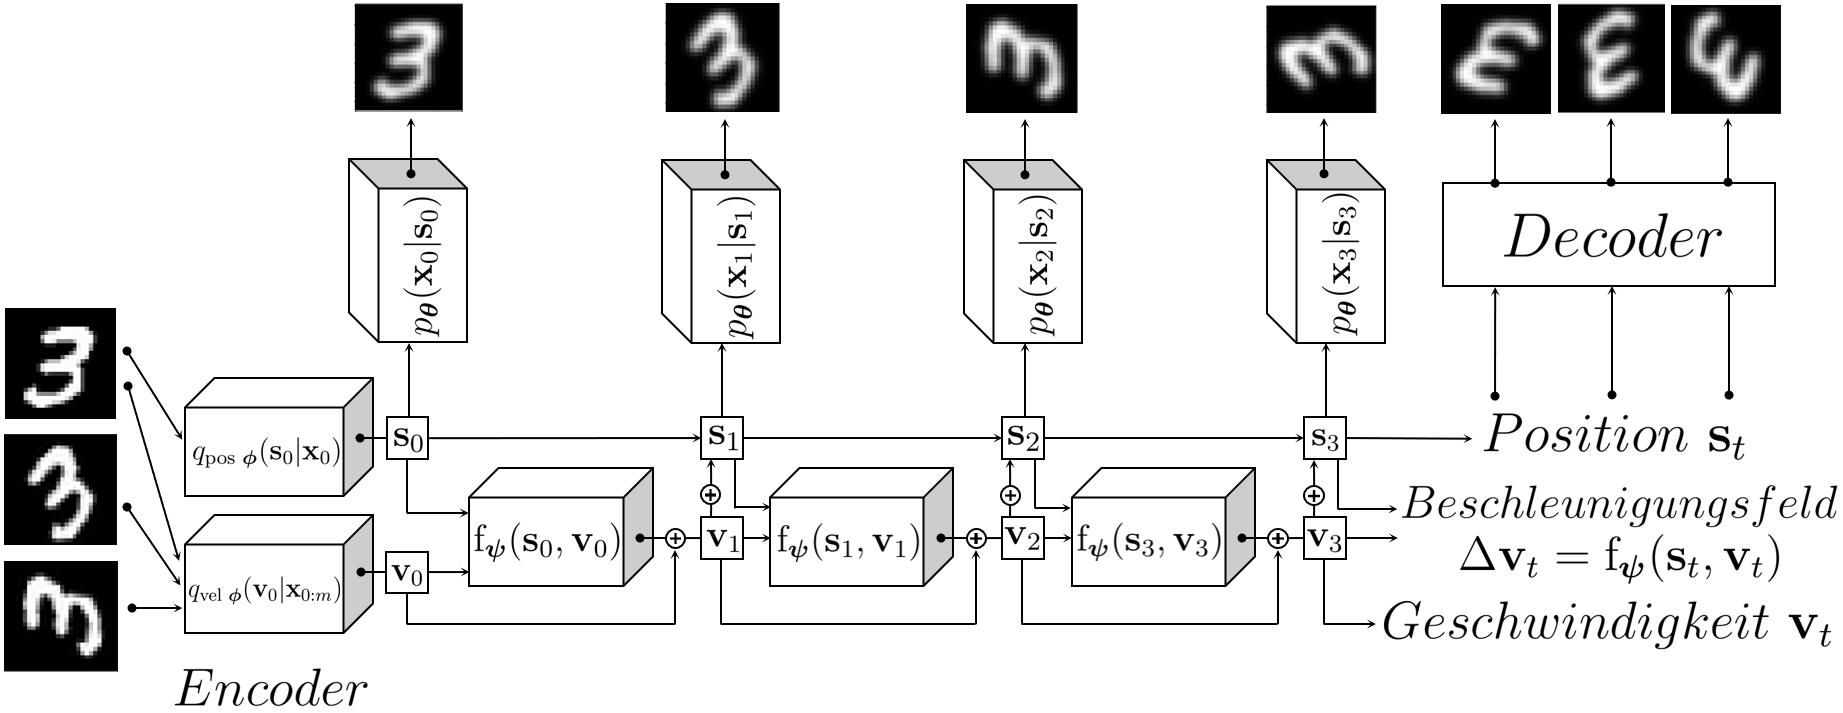
\includegraphics[scale=0.41]{ODE2VAE_Modell}
		\captionsetup{labelformat=empty}
		\caption{Das alternative Modell. Die Veränderung in der Zeit wird erneut durch das ODE-Net modelliert. Wir erhalten den Positionszustand $\mathbf{s}_{t+1} = \mathbf{s}_{t} + \mathbf{v}_{t} + f_{\boldsymbol\psi}(\mathbf{s}_{t}, \mathbf{v}_{t})$ aber durch Addition des Geschwindigkeitszustand und Auswertung des ODE-Nets, was den Rechenaufwand stark reduziert. Eine stetige Modellierung der \emph{time series} ist nun zwar nicht mehr möglich, Einbußen in der Qualität der Rekonstruktionen konnten wir aber nicht beobachten.}
	\end{figure}

	Visuell sind die Rekonstruktionen bei deutlich geringerer Trainingszeit (Bei uns ca. Faktor 30) auf unseren Datensätzen mit denen des Neural-ODE auf unseren Datensätzen vergleichbar.
	Durch Verwenden einer Summe und Simplifizierung des Trainingskriterium gehen einige praktische Eigenschaften des Modells verloren, wie das Erzeugen neuer Daten durch ziehen aus einer Normalverteilung, das Anfertigen von Rekonstruktionen in stetiger Zeit, die mathematische Interpretation des Modells als Verteilung und somit auch das Schätzen der Wahrscheinlichkeitsdichte und schließlich noch die größere Resistenz des Modells gegenüber Overfitting.
	Um einige dieser Modelleigenschaften zu erhalten könnte man auch als Trainingskriterium auch den \emph{reconstruction loss} mit der Vanilla-VAE ELBO verwenden.


	\newpage
	\subsection[SDE-VAE]{M-th Order SDE-Variational Autoencoder}
	Bisher wurden die Pfade der latenten Darstellungen $z = (s,v) : [0,\tau] \times \Omega \rightarrow \R^d$ als Lösungen von Differentialgleichungen der Form
	\begin{align*}
	\nabla s(\cdot,\omega) &= v(\cdot,\omega)\\
	\nabla v(\cdot,\omega) &= \bbf\big(s(\cdot,\omega),v(\cdot,\omega)\big)
	\end{align*}
	vorausgesetzt, wobei die 'Differential Function' $\bbf = f_\psi$ dann durch ein Neuronales Netzwerk approximiert wurde.\\
	Wir haben die folgenden Möglichkeiten in Betracht gezogen um den ODE$^2$VAE zu verallgemeinern:
	\begin{itemize}
		\item Die Pfade der latenten Darstellungen als Lösungen von Differentialgleichungen von Grad $M \geq 2$ voraussetzen. Z.B. hieße das für $M=3$:
		\begin{align*}
		\nabla s(\cdot,\omega) &= v(\cdot,\omega)\\
		\nabla v(\cdot,\omega) &= w(\cdot,\omega)\\
		\nabla w(\cdot,\omega) &= \bbf\big(s(\cdot,\omega),v(\cdot,\omega),w(\cdot,\omega)\big)
		\end{align*}

		\item Die Form der Differentialgleichung weniger einschränken, indem wir beliebige $M$-ODE zulassen.
		\begin{align*}
		\nabla s(\cdot,\omega) &= \bbf_1\big(s(\cdot,\omega),v(\cdot,\omega),w(\cdot,\omega)\big)\\
		\nabla v(\cdot,\omega) &= \bbf_2\big(s(\cdot,\omega),v(\cdot,\omega),w(\cdot,\omega)\big)\\
		\nabla w(\cdot,\omega) &= \bbf_3\big(s(\cdot,\omega),v(\cdot,\omega),w(\cdot,\omega)\big)
		\end{align*}

		\item Einen Probabilistic Encoder auf jedes Frame $x_i$ separat anwenden. Bisher wurde der Encoder nur auf die ersten Frames angewendet um $s(0,\cdot), v(0,\cdot)$ zu finden. Dies geht, wie wir später sehen werden, mit der Betrachtung von Stochastic Differential Equations (SDEs) einher.
	\end{itemize}

	\newpage
	\subsubsection[Notation]{Einführung der Notation}
	Zunächst führen wir eine Notation ein, die eher an den Standards der Stochastik und weniger an denen von Machine-Learning orientiert ist. Dazu wiederholen wir auch grob die Idee eines ODE$^2$VAE.\\
	\\
	\textbf{Idee des Autoencoders:}\\
	Sei $(\bP,\Omega,\mathcal{A})$ ein Wahrscheinlichkeitsraum mit der Zufallsvariable $x : \Omega \rightarrow \R^D$. Bei einem normalen Autoencoder wird angenommen, dass eine weitere Zufallsvariable $z: \Omega \rightarrow \R^d$ existiert, sodass $x = f(z)$ und $z = g(x)$ für messbare Funktionen $f,g$. Die Funktionen $f$ (Decoder) und $g$ (Encoder) werden dabei von Neuronalen Netzwerken anhand eines Großen Datensatzes $x^1,...,x^N \, uiv \sim (x)_*\bP$ erlernt. Als Verlustfunktion verwendet man beispielsweise den Reconstruction-Loss oder Mean Squared Error plus eventuelle Regularisierungsterme um Overfitting zu verhindern.\\
	Man stellt fest, dass der latente Raum hier eher unstrukturiert in dem Sinne ist, dass das Bildmaß $(f)_*\bP$ auf $\R^d$ vielleicht nur an ein paar Stellen den Großteil seiner Masse verteilt. An diesen Stellen im latenten Raum könnten wiederum kleine Schwankungen große Unterschiede in den Rekonstruktionen ausmachen. Anschaulich ist das Problem mit Autoencodern, dass sie den latenten Raum $\R^d$ nicht 'gleichmäßig' nutzen und man keine Kontrolle darüber hat welche Anordnungen angenommen werden.\\
	\\
	\textbf{Idee des VAE:}\\
	Einem Variational Autoencoder will man im latenten Raum eine Struktur vorgeben. $(z)_*\bP$ soll nun eine festgelegte Verteilung (z.B. Normalverteilung in $\R^d$) sein. Es müssen hier auch der Encoder $g$ und Decoder $f$ nicht mehr deterministisch sein, weshalb sie in der Literatur mit $q(z|x)$ und $p(x|z)$ beschrieben werden. Das Ziel ist erst mit Daten $x^1,...,x^N \, uiv \sim (x)_*\bP$ den Encoder und Decoder zu trainieren, um dann neue Daten generieren zu können, indem man aus der Normalverteilung $(z)_*\bP$ Werte $z^1,...,z^N$ zieht und dann den Decoder $f$ darauf anwendet.\\
	Dabei wird der Encoder als Neuronales Netzwerk aufgebaut, das im Falle einer Normalverteilung Erwartungswert $\mu(x) \in \R^d$ und Covarianzmatrix $\Sigma(x) \in \operatorname{Diag}(d\times d)$ bestimmt, bevor die latente Darstellung $z$ nach Reparametrisierung aus einer von $x$ abhängigen Verteilung, beispielsweise $g(x) = \mathcal{N}\left(\mu(x),\Sigma(x)\right)$, gezogen wird. Damit können einzelne Datenpunkte anschaulich mehr Platz im latenten Raum $\R^d$ ausfüllen. Dies lässt sich auch als Maßnahme gegen Overfitting des Encoders interpretieren.\\ Es werden neben dem Reconstruction Loss, der der Log-Likelihood entspricht mit der KL-Divergenz noch zusätzliche Terme zur Verlustfunktion addiert, die dafür zu sorgen, dass $(z)_*\bP$ eine Normalverteilung ist und dass die Verteilung $(f \circ z)_*\bP$ ähnlich der Verteilung $(x)_*\bP$ ist.

	\newpage\noindent
	\textbf{Idee des ODE$^2$VAE:}\\
	Ein ODE$^2$VAE beschäftigt sich mit Zufallsvariablen $x_0,...,x_m : \Omega \rightarrow \R^D$, bei denen angenommen wird, dass ein stetiger Prozess $\tx : [0,\tau] \times \Omega \rightarrow \R^D$ existiert, sodass $x_k = \tx_{t_k}$ für $0=t_0<...<t_m=\tau$. Der ODE$^2$VAE sucht nun einen latenten Prozess $\tz: [0,\tau] \times \Omega \rightarrow \R^d$, der punktweise die Informationen von $\tx$ encodiert, also soll der Decoder ein guter Schätzer für $\tx(t,\cdot)$ sein. Wieder wird die Struktur von $\tz$ im latenten Raum vorgeschrieben, wobei nun auch eine Vorschrift zur zeitlichen Entwicklung gemacht wird. Für spätere Zeitpunkte $t>0$ soll $\tz(t,\omega)$ als Lösung der Differentialgleichung
	\begin{align*}
	\nabla s(\cdot,\omega) &= v(\cdot,\omega)\\
	\nabla v(\cdot,\omega) &= \bbf\big(s(\cdot,\omega),v(\cdot,\omega)\big)
	\end{align*}
	nur von $s(0,\omega)$, $v(0,\omega)$ und $\bbf$ abhängen. In der Literatur wird hier das $\tz$ als gemeinsamer Vektor $(s,v)$ betrachtet. Es wird allerdings nur $s$ an den Decoder weitergeben, also soll
	%Decoder nicht als Funktion auffassen.
	 $f(s(t,\cdot))$ ein guter Schätzer für $\tx(t,\cdot)$ sein. Die Anfangswerte $s(0,\cdot)$ und $v(0,\cdot)$ werden durch jeweils einen Encoder bestimmt, die als Input $x_0$, beziehungsweise mindestens drei anfangsframes für $v(0,\cdot)$, erhalten.\\
	Die Verlustfunktion besteht aus Reconstruction-Loss, Terme um Overfitting von $\bbf$ zu verhindern, sowie Terme um $(\tz(t_k,\cdot))_*\bP$ für jedes $k \leq m$ einer Normalverteilung auf $\R^d$ näher zu bringen.\\
	Der ODE$^2$VAE liefert gute Ergebnisse beim Beschreiben von einfachen Bewegungsabläufen, deren Informationsgehalt nicht mit der Zeit zunimmt. Aber gerade bei chaotischen Systemen ist die Vorschrift, dass sämtliche Information schon zu Beginn (in den ersten drei Frames) vorhanden sein muss eher dem Lernen abträglich.\\
	Besonders ist in einem etwas chaotischerem Setting das generieren von glaubhaften Time-Series $x_0,...,x_m$ nicht möglich, da spätere $x_k, x_{k+1}$ immer deterministisch von einer gemeinsamen Zufallsvariable abhängen.\\
	\\
	\textbf{Idee des $M$-th Order SDE-VAE:}\\
	Wir beschäftigen uns wieder mit Zufallsvariablen $x_0,...,x_m : \Omega \rightarrow \R^D$, bei denen angenommen wird, dass ein stetiger Prozess $\tx : [0,\tau] \times \Omega \rightarrow \R^D$ existiert, sodass $x_k = \tx_{t_k}$ für $0=t_0<...<t_m=\tau$. Wie schon beim ODE$^2$VAE suchen wir einen latenten Prozess $\tz: [0,\tau] \times \Omega \rightarrow \R^d$,
	
	%Decoder nicht als Funktion $f(\tz(t,\cdot))$ notieren
	für den der Decoder ein guter Schätzer für $\tx(t,\cdot)$ ist. Hier gehen wir jedoch von einer anderen Zeitlichen Struktur aus.\\
	Wir schreiben $\tz = \tz^{(0)}$ und setzen voraus, dass Zufallsvariablen (Startverteilungen)
	$$\tz^{(1)}(0,\cdot) ,..., \tz^{(M-1)}(0,\cdot): \Omega \rightarrow \R^d$$
	existieren, sodass $\tz^{(k)}$ für alle $k < M$ die $d$-Dimensionale SDE
	\begin{align*}
	\forall i \leq d: \ d \big(\tz^{(k),i}(t,\cdot)\big) = & \bmu^{k,i}(\tz^{(0)}(t,\cdot),...,\tz^{(M-1)}(t,\cdot)) \, dt\\
	& \ \ + \sum\limits_{j=1}^n \bsig^{k,i,j}(\tz^{(0)}(t,\cdot),...,\tz^{(M-1)}(t,\cdot)) \, dW^j_t
	\end{align*}
	erfüllt. Dies lässt sich als eine gemeinsame SDE im Raum der $(M \times d)$-Matrizen, anstatt wie gewohnt im $\R^d$, betrachten. Wir betrachten also den Matrix-wertigen Prozess
	$$ Z_t(\omega) = \begin{pmatrix}
	\tz^{(0,1)}(t,\omega) & .. & \tz^{(0,d)}(t,\omega)\\
	: & & : \\
	\tz^{(M-1,1)}(t,\omega) & .. & \tz^{(M-1,d)}(t,\omega)
	\end{pmatrix} \in \R^{M \times d} \ .$$
	Es wird nur die Erste Zeile von $Z$ (analog zu $s$ im ODE$^2$VAE) an den Decoder weitergegeben. Die Funktionen $\bmu : \R^{M \times d} \rightarrow \R^{M \times d}$ und $\bsig : \R^{M \times d} \rightarrow \R^{M \times d \times n}$ werden mit Neuronalen Netzwerken gelernt.\\
	Das Ziel hierbei ist nicht diese Lösung direkt in einen Encoder einzugeben um die eingegebenen Daten zu rekonstruieren, sondern anhand des gelernten $\bmu$ eine ODE ohne 'Unsicherheit' $\bsig$ zu simulieren. Diese glatte Lösung der ODE kann dann in die Decoder eingegeben um anschaulich geglättete oder weniger chaotische Daten zu erhalten.\\
	Interessant ist, dass beim Training die originalen, ungeglätteten latenten Darstellungen $\tz^{(0)}(t_0,\cdot),...,\tz^{(0)}(t_m,\cdot)$ in die Decoder eingegeben werden. Zusätzliche Verlustfunktionen sorgen dafür, dass $\bmu, \bsig$ erlernt werden sowie dass die En-\&Decoder lernen $z$ als SDEs darzustellen.\\
	Die erlernten $\bmu,\bsig$ können verwendet werden um neue Pfade von $Z$ zu ziehen (simulieren), mit denen man glaubhaft neue Daten generieren kann.\\
	\\
	Der ODE$^2$VAE ist nur ein einfacher Spezialfall dieser Darstellung. Wenn wir nämlich $M=2$, $\bsig = 0$ und $\bmu^{(0)}(\tz^{(0)},\tz^{(1)}) = \tz^{(1)}$ setzen, dann erfüllt $\bmu^{(0)}(\tz^{(0)},\tz^{(1)})$ dieselbe Rolle, wie $\bbf$ im ODE$^2$VAE.\\
	\\
	Damit man mit dem Modell besser neue Daten generieren kann, soll $(\tz(0,\cdot))_*\bP$ wie beim VAE und beim ODE$^2$VAE in die Form einer Normalverteilung auf $\R^d$ gezwungen werden. Leider hatten wir nicht mehr genug Zeit die ELBO in diesem Fall herzuleiten und arbeiten mit provisorischen Verlustfunktionen für das neue Modell.
	Man könnte daher argumentieren, dass unser Modell teilweise eher einem Autoencoder ähnelt, als einem Variational Autoencoder.






	\newpage
	\subsubsection[Lernen von SDEs]{Lernen von SDEs}
	Sei $\bmu: \R^d \rightarrow \R^d$ und $\bsig: \R^d \rightarrow \R^{d \times n}$. Für Prozesse $X: [0,\tau] \times \Omega \rightarrow \R^d$ und $W^1,...,W^n : [0,\tau] \times \Omega \rightarrow \R$ heißt $(Z,W)$ starke Lösung der Stochastischen Differentialgleichung (SDE)
	\begin{align*}
		& dZ^i = \bmu^i(t,Z_t) \, dt + \sum\limits_{j=1}^n \bsig^{i,j}(t,Z_t) \, dW^j \ ,
	\end{align*}
	falls $W^1,...,W^n$ unabhängige Brownsche Bewegungen sind und die Formel
	\begin{align*}
		& Z_t^i - Z_0^i = \int_0^t \bmu^i(s,Z_s) \, ds + \sum\limits_{j=1}^n \int_0^t \bsig^{i,j}(s,Z_s) \, dW_s^j \tag{1}
	\end{align*}
	für jedes $i \leq d$ erfüllt ist. Wir sind hier nur an dem Fall, dass $\bmu(t,x)$ und $\bsig(t,x)$ nicht von $t$, sondern nur von $x$ abhängen, interessiert. Die Lösungen solcher SDEs nennt man Ito-Diffusionen.\\
	Nach \cite{PfaffiSkript} Thm. 21.4 existiert unter den Voraussetzungen
	\begin{align*}
		& ||\bmu(x)||_2 + ||\bsig(x)||_2 \leq C_1 \, (1+||x||_2)\\
		& ||\bmu(x)-\bmu(y)||_2 + ||\bsig(x)-\bsig(y)||_2 \leq C_2 \, ||x-y||_2 \tag{2}
	\end{align*}
	für jede Startverteilung $Z_0$ mit endlichem zweiten Moment und beliebige Brownsche Bewegungen. $W^1,...,W^n$ eine eindeutige Lösung $Z = Z(W)$ der oben beschriebenen SDE.\\
	Mit Hilfe des Euler-Maruyama-Verfahrens lässt sich diese Lösung approximieren. Dazu Teilen wir das Intervall $[0,\tau]$ in $m$ viele Stücke $[t^m_k,t^m_{k+1}]$ mit $\Delta t = \frac{\tau}{m}$ und $t^m_k = k \Delta t^m = \frac{k\tau}{m}$. Wir definieren rekursiv
	\begin{align*}
		& Z^i_{m,t^m_k} := Z^i_{m,t^m_{k-1}} + \bmu^i(Z_{m,t^m_{k-1}}) \, \Delta t + \sum\limits_{j=1}^n \bsig^{i,j}(Z_{m,t^m_{k-1}}) \, \underbrace{(W^j_{t_k}-W^j_{t_{k-1}})}_{\sim \mathcal{N}(0,\Delta t)}
	\end{align*}
	mit $Z_{m,0} = Z_0$. Da Brownsche Bewegungen unabhängige Segmente haben, können wir analog $(\varepsilon_{j,k})_{j \leq n, k \in \N} \, uiv. \sim N(0,1)$ definieren und schreiben:
	\begin{align*}
		& \tZ^i_{m,t^m_k} := \tZ^i_{m,t^m_{k-1}} + \bmu^i(\tZ_{m,t^m_{k-1}}) \, \Delta t^m + \sum\limits_{j=1}^n \bsig^{i,j}(\tZ_{m,t^m_{k-1}}) \, \sqrt{\Delta t^m} \, \varepsilon_{j,k} \ .
	\end{align*}
	Solche $\tX_m$ lassen sich nun leicht mit dem Computer generieren und wir wissen nach Euler-Maruyama, dass ein $c > 0$ existiert, sodass für jedes $t \in [0,\tau]$ gilt:
	\begin{align*}
		& \E[||Z_{m,t} - Z_t||_2] \leq \frac{c}{\sqrt{m}} \ .
	\end{align*}

	\newpage
	\noindent
	Ein einfacher Weg nun die Funktionen $\bmu$ aus Realisierungen von $(Z_{t^m_0},...,Z_{t^m_m})$ approximativ zu lernen ist nun aus der Sicht des Computers den Prozess $Z$ mit seiner Euler-Maruyama Arpproximation $Z_m$ gleich zu setzten. Man würde also annehmen, dass $Z_{t^m_k} = Z_{m,t^m_k}$ mit
	\begin{align*}
	& Z^i_{m,t^m_k} = Z^i_{m,t^m_{k-1}} + \bmu^i(Z_{m,t^m_{k-1}}) \, \Delta t^m + \sum\limits_{j=1}^n \bsig^{i,j}(Z_{m,t^m_{k-1}}) \, \sqrt{\Delta t^m} \, \varepsilon_{j,k} \ .
	\end{align*}
	Wenn man nun $\bmu$ und $\bsig$ lernen wollte, indem man versucht mit der rechten Seite der Gleichung die linke Seite vorherzusagen, würde nur $\bmu$ richtig trainiert werden. Um $\bsig$ richtig zu trainieren nutzen wir etwas mehr Theorie.\\
	\\
	Die Quadratische Variation und Covariation von Semimartingalen werden in \cite{PfaffiSkript} Prop. 19.28 und Thm. 19.31 definiert. Nach Lemma 19.50 wissen wir, dass
	\begin{align*}
	& \sum\limits_{k=1}^m (Z^i_{t^m_{k}}-Z^i_{t^m_{k-1}})(Z^l_{t^m_{k}}-Z^l_{t^m_{k-1}}) \xrightarrow{m \rightarrow \infty}_p [Z^i,Z^l]_\tau
	\end{align*}
	Weiter wissen wir nach den Eigenschaften der Covariation und $Z$, dass
	\begin{align*}
	& [Z^i,Z^l]_\tau = \left[ \int_0^\tau \bmu^i(Z_s) \, ds + \sum\limits_{j=1}^n \int_0^\tau \bsig^{i,j}(Z_s) \, dW_s^j, \int_0^\tau \bmu^l(Z_s) \, ds + \sum\limits_{j=1}^n \int_0^\tau \bsig^{l,j}(Z_s) \, dW_s^j \right]\\
	& \overset{19.44\&19.45}{=} \left[ \sum\limits_{j=1}^n \int_0^\tau \bsig^{i,j}(Z_s) \, dW_s^j, \sum\limits_{j=1}^n \int_0^\tau \bsig^{l,j}(Z_s) \, dW_s^j \right]\\
	& = \sum\limits_{j,j'=1}^n \left[ \int_0^\tau \bsig^{i,j}(Z_s) \, dW_s^j, \int_0^\tau \bsig^{l,j'}(Z_s) \, dW_s^{j'} \right]\\
	& \overset{19.37}{=} \sum\limits_{j,j'=1}^n \int_0^\tau \bsig^{i,j}(Z_s)\bsig^{l,j'}(Z_s) \, d\underbrace{\left[W^j, W^{j'} \right]_s}_{=1_{j=j'} \, s} = \sum\limits_{j=1}^n \int_0^\tau \bsig^{i,j}(Z_s)\bsig^{l,j}(Z_s) \, ds
	\end{align*}
	Indem wir nun den unteren Term durch $A_{i,l} := \sum\limits_{j=1}^n \Delta t^m \sum\limits_{k=1}^m \bsig^{i,j}(Z_{t_k})\bsig^{l,j}(Z_{t_k})$ und den oberen Term $[Z^i,Z^l]_\tau$ wie in der oberen Überlegung durch $B_{i,l} := (Z^i_{t^m_{k}}-Z^i_{t^m_{k-1}}) (Z^l_{t^m_{k}}-Z^l_{t^m_{k-1}})$ approximieren, können wir die ganze Matrix $\bsig \in \R^{d \times n}$ trainieren, indem wir den Abstand zwischen $A$ und $B$ bestrafen.\\
	Wir trainieren hier effektiv nur $\bsig \bsig^* \in \R^{d \times d}$, aber viel besser kann man $\bsig$ auch nicht bestimmen, da man z.B. bei zwei unabhängigen Brownschen Bewegungen $W^1,W^2$ man nicht zwischen $\sqrt{2}W_1, W_1+W_2, W_1-W_2, \sqrt{2}W_2$ anhand ihrer Verteilung unterscheiden kann.
	
	
	\newpage
	\subsubsection[Modell]{Aufbau des $M$-SDE-VAE-Modells}
	Sei $(\bP, \Omega, \mathcal{A})$ ein Wahrscheinlichkeitsraum und $\tx : [0,\tau] \times \Omega \rightarrow \R^D$ ein stetiger Prozess. Für $0=t_0<...<t_m=\tau$ definieren wir die Zufallsvariablen $x_k := \tx(t_k,\cdot)$. Wir gehen der Einfachheit halber davon aus, dass die Abstände $t_k-t_{k-1}$ alle gleich sind, also $t_k = k\frac{\tau}{m} = k \, \Delta t$.\\
	Gegeben seien Daten $(x_1^p,...,x_m^p)_{p \in \N}\, uiv. \sim (x_1,...,x_m)_*\bP$. Wir definieren einen Encoder $g: \R^D \rightarrow \R^d$ und einen Decoder $f: \R^d \rightarrow \R^D$ für $d<<D$. Dabei ist $g(x)$ gegeben $x$ nicht deterministisch, sondern wird (bedingt) unabhängig aus einer $d$-dimensionalen Normalverteilung $\mathcal{N}(\mu(x),\Sigma(x))$ gezogen. Wir schreiben formell $\bP(g(x_k) \mid x_k) = \mathcal{N}(\mu(x_k),\Sigma(x_k))$ für alle $k \leq m$.\\
	Die Funktionen $\mu: \R^d \rightarrow \R^d$, $\Sigma: \R^d \rightarrow \operatorname{Diag}(d \times d)$ sowie $f: \R^d \rightarrow \R^D$ werden durch CNNs dargestellt. Für unseren genauen Aufbau für Anwendung auf den rotating-MNIST Datensatz siehe Sektion 4.\\
	Wir definieren die Zufallsvariablen $z_0,...,z_m : \Omega \rightarrow \R^{d}$ durch $z_k = z^{(0)}_k := g(x_k)$. Analog benennen wir die encodierten Daten $z_k^p(\omega) = z_k^{(0),p}(\omega) := g_\omega(x_k^p(\omega))\in \R^d$.\\
	Wir wollen $z^{(0)}_k$ interpretieren, als seien sie Momentaufnahmen
	$$z^{(0)}_k = \tz^{(0)}(t_k,\cdot) = ( \tz^{(0,1)}(t_k,\cdot),...,\tz^{(0,d)}(t_k,\cdot))$$
	eines Prozesses
	$$ Z_t(\omega) = \begin{pmatrix}
	\tz^{(0,1)}(t,\omega) & .. & \tz^{(0,d)}(t,\omega)\\
	: & & : \\
	\tz^{(M-1,1)}(t,\omega) & .. & \tz^{(M-1,d)}(t,\omega)
	\end{pmatrix} \in \R^{M \times d} \ ,$$
	der die Lösung eine noch unbekannten SDE ist. Um die SDE zu lernen, definieren wir $\bmu : \R^{M \times d} \rightarrow \R^{m \times d}$ und $\bsig: \R^{M \times d} \rightarrow \R^{m \times d \times n}$ als Neuronale Netzwerke. Um diese Netzwerke trainieren zu können, benötigen wir auch für $0<l<M$ empirische Daten $(z_1^{(l),p},...,z_m^{(l),p})_{p \in \N}$. Diese könnten durch weitere Encoder entstehen, wie es bereits im 2-ODE-VAE für den Startwert $v(0,\cdot)$ gemacht wird. Falls $M$ eher klein ist, oder von einer geringen 'Unsicherheit' $\bsig$ ausgegangen werden kann, kann man die $(z_1^{(l),p},...,z_m^{(l),p})_{p \in \N}$ auch als empirische Ableitungen $z_k^{(l),p} := \frac{1}{\Delta t} \, (z_{k+1}^{(l-1),p} - z_k^{(l-1),p}) \in \R^d$ definieren. Die Vorstellung als Annäherung einer Ableitung ist hier eigentlich falsch, da Lösungen von SDEs mit positivem $\bsig$ nirgends differenzierbar sind, aber wie wir schon bei der Theorie zum Lernen von SDEs gesehen hatten, ist $\E[\frac{1}{\Delta t} \, (z_{k+1}^{(l-1),p} - z_k^{(l-1),p}) \mid z_k^{(l-1),p}] \approx \bmu(z_k^{(l-1),p})$, also eignen die $z_k^{(l),p}$ sich zumindest bei großen Datensätzen um SDEs höherer Ordnung zu lernen.
	
	\newpage
	\noindent
	
	Für unser Modell definieren wir und nun einen 'Reconstructor' $R_{\bmu,\bsig} : \R^{M \times d} \rightarrow \prod\limits_{k=0}^m \R^{M \times d}$, der zu gegebenen Anfangswerten $(z^{0}_0,...,z^{M-1}_0) = Z_0$ mit Hilfe der Funktionen $\bmu, \bsig$ das Euler-Maruyama-Verfahren anwendet um $Z_{m,t_1},...,Z_{m,t_m} \in \R^{M \times d}$ (Notation aus Theorie zum Lernen von SDEs) nacheinander zu Konstruieren.\\
	Wir verwenden dabei zur Rekonstruktion besonders $R_{\bmu,0}$, da für $\bsig = 0$ das Euler-Maruyama-Verfahren mit dem Euler-Verfahren übereinstimmt und wir damit $z_{1,rec}^{(l),p},...,z_{m,rec}^{(l),p} := Z_{m,t_1},...,Z_{m,t_m}$ glatter als die eingegebenen $z_1^{(l),p},...,z_m^{(l),p}$ rekonstruieren können.\\
	\\
	Wir definieren die folgenden Verlustfunktionen:
	\begin{itemize}
		\item Reconstruction-Loss:
		\begin{align*}
		& L_r := H\big((x_0,...,x_m)_*\bP, (f(z_0^{(0)}),...,f(z_m^{(0)})_*\bP)\big)
		\end{align*}
		Dabei steht $H$ für die Binäre Kreuzentropie zwischen den Verteilungen.
		
		\item Latent-Reconstruction-Loss:
		\begin{align*}
		& L_{lr} := \E\left[\left( \sum\limits_{k=0}^m \sum\limits_{i=1}^d (z^{(0,i)}_k-z^{(0,i)}_{k,rec})^2 \right)^{\frac{1}{2}}\right]
		\end{align*}
		
		\item Latent-Pointwise-Loss:
		\begin{align*}
		& L_{lp} := \E\left[\left( \sum\limits_{k=0}^{m-1} \sum\limits_{l=1}^{M-1} \sum\limits_{i=1}^d \big(\bmu^{l,i}(z_k) - \Delta t (z^{(l-1,i)}_{k+1} - z^{(l-1,i)}_{k}) \big)^2 \right)^{\frac{1}{2}}\right]
		\end{align*}
		
		\item Latent-Covariance-Loss:
		Wir betrachten die oben definierten $Z_{t_k}$ als Vektoren in $\R^{Md}$. Seien $A_{i,l}$ und $B_{i,l}$ wie sie in der Theorie zum lernen von SDEs definiert werden.
		\begin{align*}
		& L_{lcv} := \E\left[\left( \sum\limits_{i,l=1}^d \big( A_{i,l}-B_{i,l} \big)^2 \right)^{\frac{1}{2}}\right]
		\end{align*}
		
		
	\end{itemize}
	Während des Trainings werden diese Verlustfunktionen, die eigentlich von den Zufallsvariablen $(x_0,...,x_m)$ abhängen, Batch-weise als Mittelwert über die gegebenen Daten $(x_1^p,...,x_m^p)_{p \in \N}\, uiv. \sim (x_1,...,x_m)_*\bP$ approximiert. Die Gewichtung der Verlustfunktionen muss vom Datensatz abhängig gewählt werden. 
	
	
	





	\newpage
	\section[Empirische Untersuchung]{Empirische Untersuchung}
	\subsection[Datensätze]{Die verwendeten Datensätze}
	\subsubsection{Rotating MNIST}
	\begin{figure}[!htbp]
		\centering
		
\includegraphics[scale=0.4]{rotatingMNIST}
	\end{figure}
	Bei dem Datensatz \emph{rotatingMNIST} handelt es sich um eine Modifikation des bekannten MNIST-Datensatzes. Die Grauwerte der Bilder
	des MNIST-Datensatzes wurden von uns zunächst binärisiert, um durch eine Bernoulli-Verteilung im Decoder dargestellt werden zu können.
	Hierbei wurden die Farbwerte 0 bis 127 auf den Wert 0 abgebildet und die Werte 128 bis 255 auf den Wert 1. \\
	Ein Datenpunkt $\x\in \{0,1\}^{28\times 28\times 10}$ aus dem Datensatz enthält eine Sequenz von 10 Frames, von einem Frame auf das nachfolgende Frame rotiert die entsprechende Ziffer um 36$^\circ$ gegen den Uhrzeigersinn. Insgesamt wird so eine Rotation um 360$^\circ$ dargestellt. \\
	Der Trainingsdatensatz besteht aus 60000 Sequenzen und der Testdatensatz aus 10000 Sequenzen. Der Code zum erzeugen des Datensatz wurde von uns selbst geschrieben und erlaubt es, falls gewünscht auch eine andere Frameanzahl festzulegen.

	\subsubsection{Bouncing Balls}
	\begin{figure}[!htbp]
		\centering
		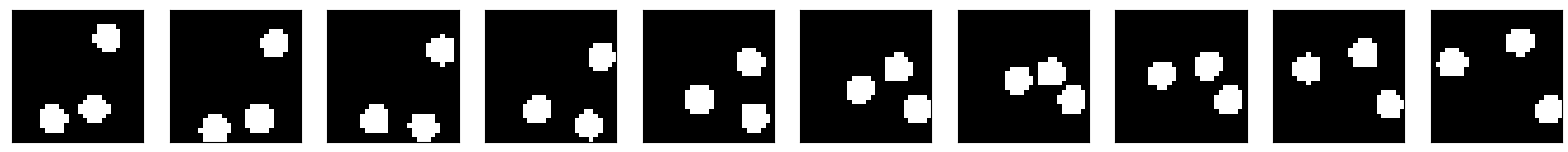
\includegraphics[scale=0.4]{bouncingBalls}
	\end{figure}
	Der Datensatz \emph{bouncingBalls} besteht aus Bildsequenzen, die Bewegungen dreier gleichgroßer zweidimensionaler Bälle enthalten. Die Bälle befinden sich zum Anfangszeitpunkt in zufälliger Position im Bild und bewegen sich mit normiertem Beschleunigungsvektor in zufällige Richtungen. Dabei können sie miteinander und den Bildrändern kollidieren.
	Die zugrundeliegenden physikalischen Gesetze einer elastischen Kollisionen zwischen den Bällen und mit den Bildrändern können in \cite{ElastKol} nachgelesen werden und sollen von unserem Modell erlernt werden. \\
	Ein Datenpunkt $\x\in \{0,1\}^{28\times 28\times 10}$ aus dem Datensatz enthält 10 Frames. Der Wert 1 bedeutet, dass sich an der jeweiligen
	Stelle auf dem Frame ein Ball befindet.\\
	Obwohl dieser Datensatz dem des Papers zum ODE$^2$VAE sehr ähnelt ist er für das Modell komplexer zu erlernen, da bei uns zum einen weniger Frames enthalten sind, zwischen diesen aber mehr Zeit vergeht.\\
	Der Trainingsdatensatz besteht aus 60000 Sequenzen und der Testdatensatz aus 10000 Sequenzen.
	Der Code zum erzeugen des Datensatz wurde von uns selbst geschrieben und ermöglicht es, falls erwünscht auch eine andere Anzahl der Bälle, Frames, Auflösung und unterschiedlichen Radius zu wählen.

	\subsubsection{AVI-Motion}
	\begin{figure}[!htbp]
		\centering
		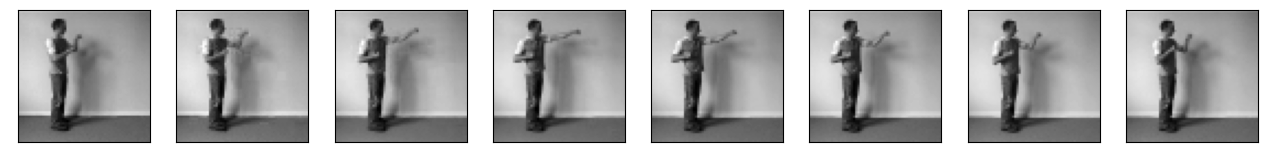
\includegraphics[scale=0.5]{AVIMotion}
	\end{figure}
	Der Datensatz \emph{AVI-Motion} besteht aus Bildsequenzen, die drei menschliche Bewegungen (klatschen, boxen und winken) darstellen. Der ursprünglische Datensatz enthält zu diesen Bewegungen je 4 Videosequenzen von jeweils 25 unterschiedlichen Personen, die jeweils mehrere Sekunden lang sind und eine Auflösung von $160\times120$ Pixel haben. Der Datensatz kann von der Website \cite{Dataset} heruntergeladen werden.
	Wir haben die Videosequenzen auf eine Auflösung von $60\times60$ reduziert, indem wir die Personen mittig in einem $120\times120$ großen Ausschnitt zentiert haben und die Auflösung schließlich durch Mean-Pooling verringert haben. \\
	Ein Datenpunkt $\x\in [0,1]^{60\times 60\times 8}$ enthält 8 Frames. Die Farbwerte sind stetige Grauwerte zwischen 0 (schwarz) und 1 (weiß). Wir wollen auf diesem Datensatz testen, ob sich das Modell des ODE$^2$VAE dazu eignet, reale Videosequenzen zu modellieren.\\
	Der Trainingsdatensatz besteht dazu aus 17472 Sequenzen und der Testdatensatz aus 112 Sequenzen. Im Gegensatz zu den anderen Datensätzen legen wir die Batchsize hier auf $M=112$ fest (da $112 | 17472$).

	\subsubsection{SDE Ball}
		\vspace{-0.4cm}
	\begin{figure}[!htbp]
		\centering
		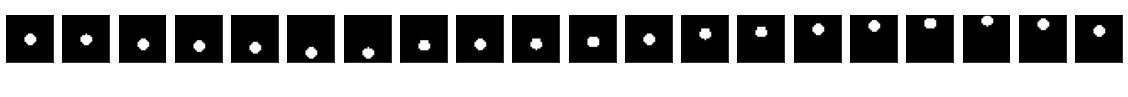
\includegraphics[scale=0.405]{datasetSDE}
	\end{figure}
	\vspace{-0.3cm}
	Dieser einfache Datensatz zeigt einen Ball, der sich nach dem Pfad einer SDE mit einer Brownschen Bewegung ($n=1$) nach oben und unten bewegt. Die SDE von Grad $2$ hat die Form
	\begin{align*}
	& \bmu: \R^{2} \rightarrow \R^{2} \ ; \ \bmu(x,y) = (y,-x)\\
	& \bsig : \R^{2} \rightarrow \R^{2 \times 1} \ ; \ \bsig(x,y) = (0.2, 0.1) \ .
	\end{align*}
	Für die Position des Balls wird nur die erste Koordinate der Lösung der SDE betrachtet. Falls $\bsig$ gleich $0$ wäre, würde es sich hierbei um die Differentialgleichung handeln, deren Lösung durch Sinus und Kosinus gegeben sind. Der Pfad des Balls beschreibt also anschaulich eine 'chaotische' Sinuskurve. Als Startwert der SDE wird immer $(0,1)$ gewählt.\\
	Ein Datenpunkt $\x\in \{0,1\}^{28\times 28\times 50}$ aus dem Datensatz enthält 50 Frames.
	Der Trainingsdatensatz besteht aus 3000 Sequenzen und der Testdatensatz aus 1000 Sequenzen.

	\subsection[Ergebnisse]{Ergebnisse}
	\subsubsection{Methode 1: Lineare Interpolation im latenten Raum}
	\begin{figure}[h!]
		\begin{center}
		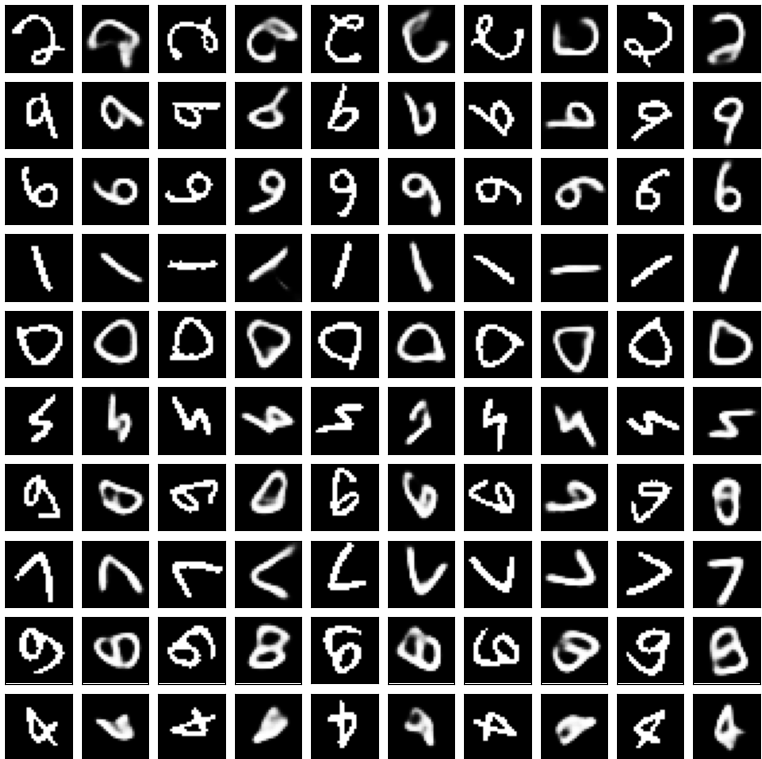
\includegraphics[scale=0.55]{interpolation}
		\end{center}
	\end{figure}
	In der Abbildung sehen wir zehn Bildsequenzen aus dem Datensatz rotatingMNIST. Die Bilder zu den Zeitpunkten $t=0,2,4,6,8$ sind Modellinput und die Bilder den Zeitpunkten $t=1,3,4,7,9$ sind Rekonstruktionen der fehlenden Bilder mittels linearer Interpolation im latenten Raum. \\
	Das Modell wird auf den Datenpunkten für 50 Epochen trainiert, indem die time series $\mathbf{x}_{0:T}$ in voneinander unabhängige Datenpunkte $\{\mathbf{x}_t\}_{i=0}^T$ aufgeteilt werden.
	Um die fehlenden Bilder zu rekonstruieren, werden die vom Decoder bestimmten latenten Darstellungen durch eine Gerade $\z_{t+1} = \z_t + a(\z_{t+2}-\z_t)$ verbunden, welche zum gewünschten Zeitpunkt, bei uns $a = 0.5$ und $a = 1.5$ für $t=9$, ausgewertet wird. 
	Das Ergebnis wird als latente Darstellung für das fehlendene Bild verwendet und mithilfe des Decoders rekonstruiert. \\
	Theoretisch lassen sich so zwischen zwei Bildern beliebig viele Rekonstruktionen anfertigen.\\
	Auffallend ist, dass diese Methode nicht immer gute Rekonstruktionen liefert. 
	Je nach Sequenz schwanken die Rekonstruktionen zwischen minimalen Abweichungen bis hin zu stark verschwommenen oder falsch rekonstruierten Bildern. Hierbei können wir gut sehen, dass die Cluster im latenten Raum 
	nicht immer konvex angeordnet sind. So wird beispielweise im linken Bild bei der siebten und 
	neunten Sequenz eine 9 zu einer 0 bzw. einer 8 rekonstruiert. Sobald ein Cluster eine annähernd konvexe Form hat erhalten wir, wie beispielweise in der 
	dritten, vierten, fünften oder achten Sequenz, eine gute Rekonstruktion. Die Methode ist daher auf Datensätzen mit vielen Eigenschaften, oder mit Bildern, die in ihren Eigenschaften zu weit auseinanderliegen ungeeignet, da die Interpolationsgerade oft auch durch ein anderes Cluster geht.
	\\
	\subsubsection{Methode 2: Vanilla-VAE}
		\begin{figure}[h!]
		\begin{minipage}{0.32\textwidth}
%			\begin{mdframed}[style=inner]
				\center{Modellinput\vspace{0.1cm}}
				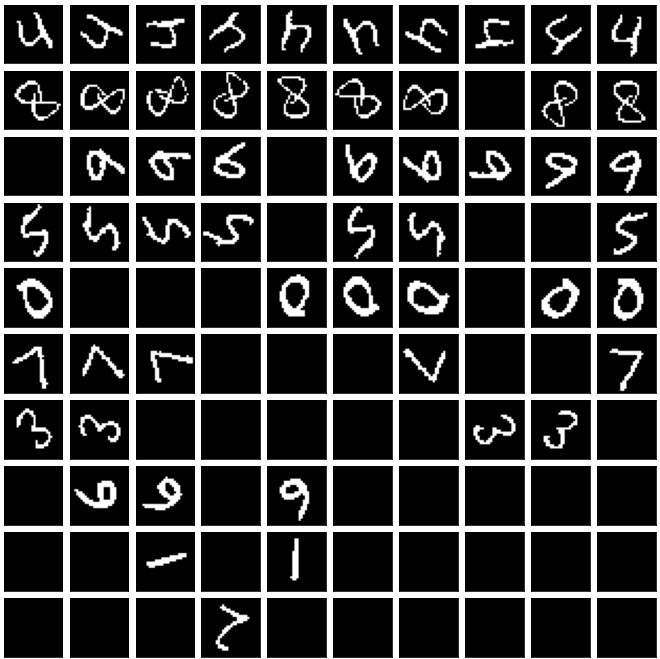
\includegraphics[scale=0.22]{rotatingMNIST_VAE}
%			\end{mdframed}
		\end{minipage}
		\begin{minipage}{0.32\textwidth}
%		\begin{mdframed}[style=inner]
			\center{Trainingsdaten vollständig\vspace{0.1cm}}
			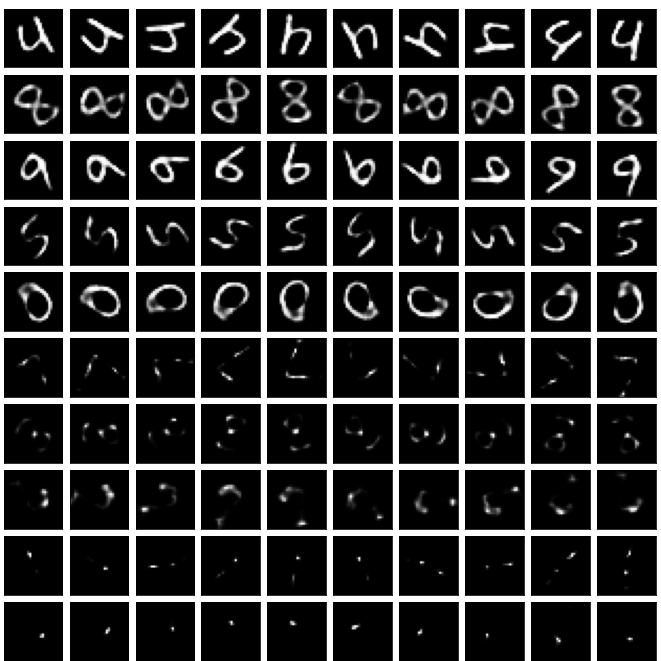
\includegraphics[scale=0.22]{rotatingMNIST_VAElat}
%		\end{mdframed}
		\end{minipage}
		\begin{minipage}{0.32\textwidth}
%			\begin{mdframed}[style=inner]
				\center{Trainingsdaten beschädigt\vspace{0.1cm}}
				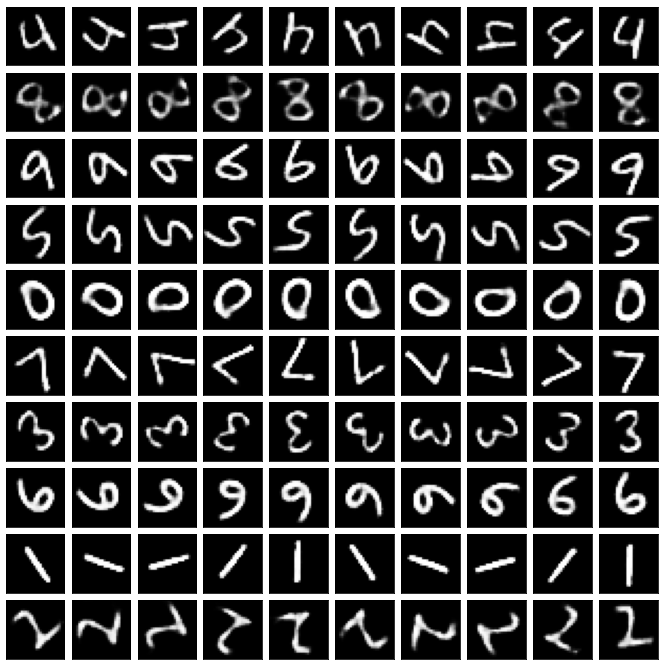
\includegraphics[scale=0.22]{rotatingMNIST_VAElat2}
%			\end{mdframed}
		\end{minipage}
%		\caption{Blablabla}

	\begin{minipage}{0.32\textwidth}
		%			\begin{mdframed}[style=inner]
		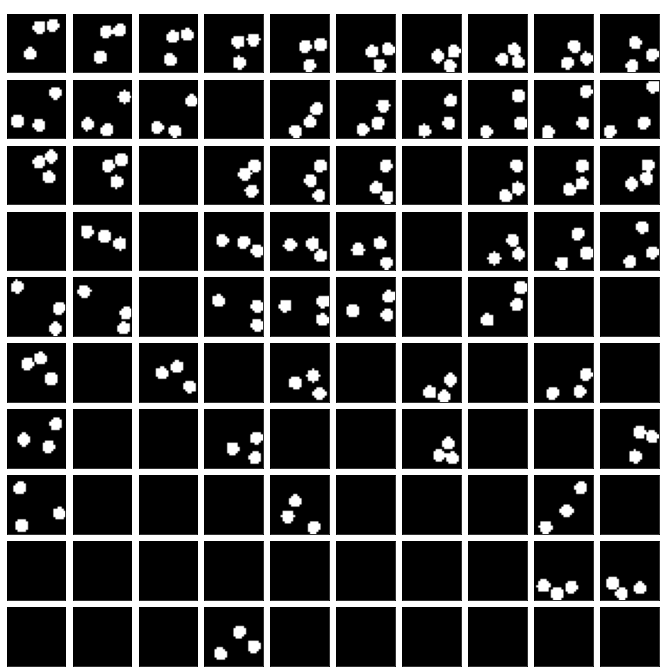
\includegraphics[scale=0.22]{bouncingBalls_VAE}
		%			\end{mdframed}
	\end{minipage}
	\begin{minipage}{0.32\textwidth}
		%		\begin{mdframed}[style=inner]
		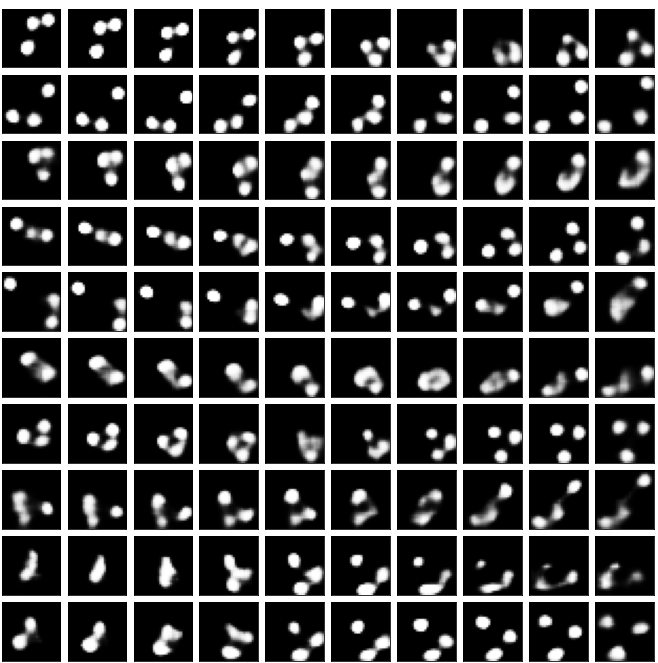
\includegraphics[scale=0.22]{bouncingBalls_VAElat}
		%		\end{mdframed}
	\end{minipage}
	\begin{minipage}{0.32\textwidth}
		%			\begin{mdframed}[style=inner]
		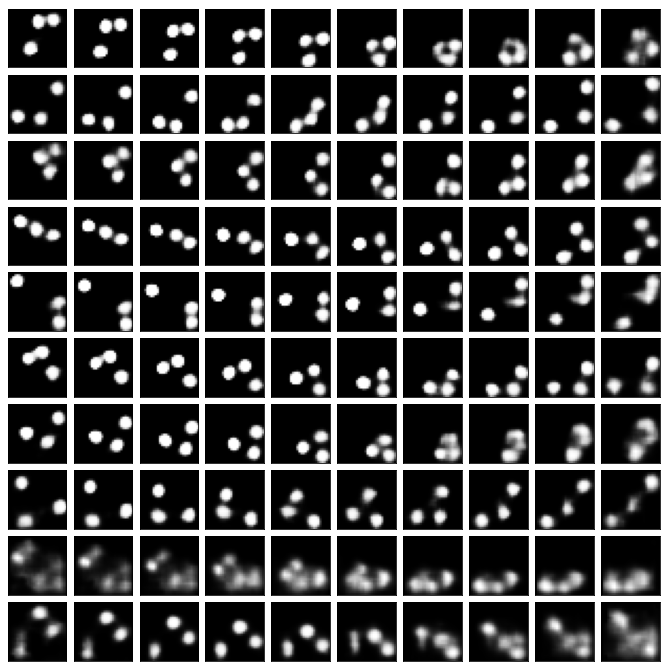
\includegraphics[scale=0.22]{bouncingBalls_VAElat2}
		%			\end{mdframed}
	\end{minipage}
	%		\caption{Blablabla}
	\end{figure}
	In den sechs Abbildungen sehen wir je zehn Bildsequenzen aus den Datensätzen rotatingMNIST und bouncingBalls. 
	Ganz Links ist der Modellinput abgebildet. Wir haben aus diesem jeweils 0 bis 9 Frames entfernt, die von unserem Modell rekonstruiert werden sollen.\\
	Dafür haben wir einen VAE für 100 Epochen auf den Datensätzen trainiert, wobei die time series als gesamtes als Modellinput verwendet.\\
	Mittig sind die Rekonstruktionen eines VAE abgebildet, der auf einem unbeschädigten Datensatz trainiert wurde und nach dem Training beschädigte Sequenzen des Testdatensatz rekonstruieren sollte. Die Idee dahinter ist, dass dem Modell diese Daten unbekannt sind und sie nach Abbildung in den latenten Raum daher vom Decoder vollständig rekonstruiert werden.
	Die Rekonstruktionen werden dabei aber immer schlechter, je mehr Daten aus dem ursprünglichem Bild fehlen. \\
	Wir behelfen uns daher mit einem Trick. Wir beschädigen auch den Trainingsdatensatz, trainieren den VAE aber darauf die gesamte Sequenz und nicht das beschädigte Inputbild zu rekonstruieren. Wie man in den Abbildungen rechts erkennen kann führt das zu einer deutlichen Verbesserung der Modellperformance.\\


%	\begin{figure}[!htbp]
%		\centering
%		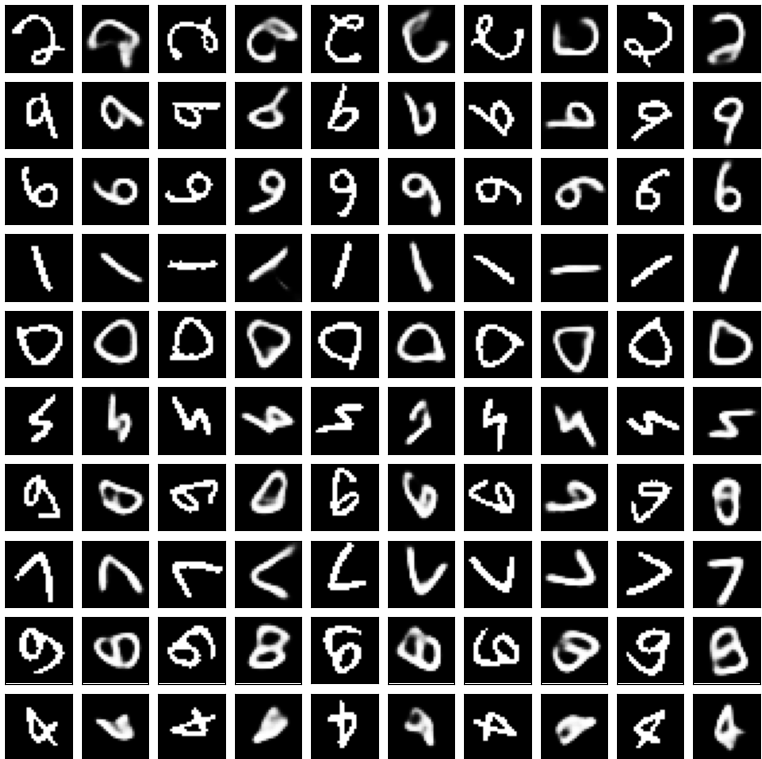
\includegraphics[scale=0.8]{interpolation}
%		\caption{Rekonstruktion der \emph{time series} mittels VAE mit Interpolation.}
%		\label{Abb:VAEmitInterpol}
%	\end{figure}

%	\begin{figure}[!htbp]
%		\centering
%		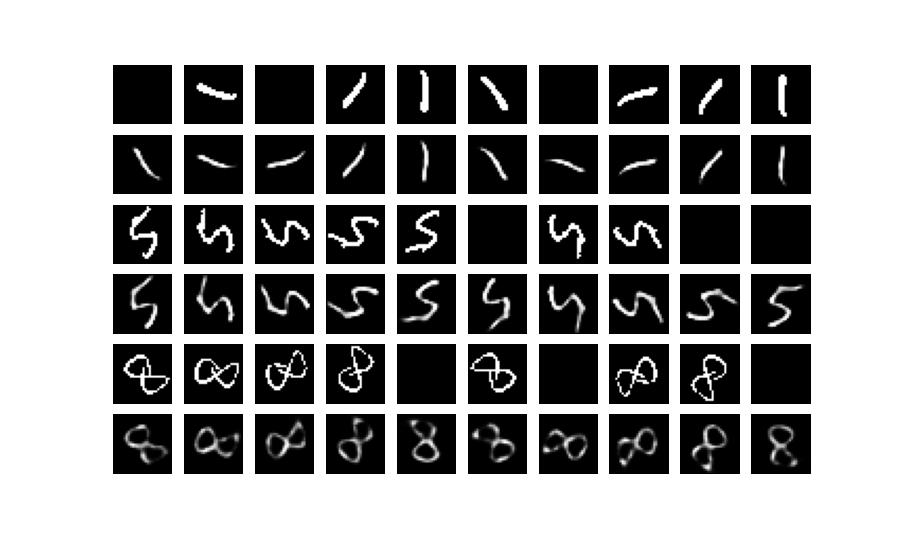
\includegraphics[scale=0.8]{whole_sequence_mnist}
%		\caption{Rekonstruktion der \emph{time series} mittels VAE ohne Interpolation.}
%		\label{Abb:VAEohneInterpolMNIST}
%	\end{figure}
%	\begin{figure}[!htbp]
%		\centering
%		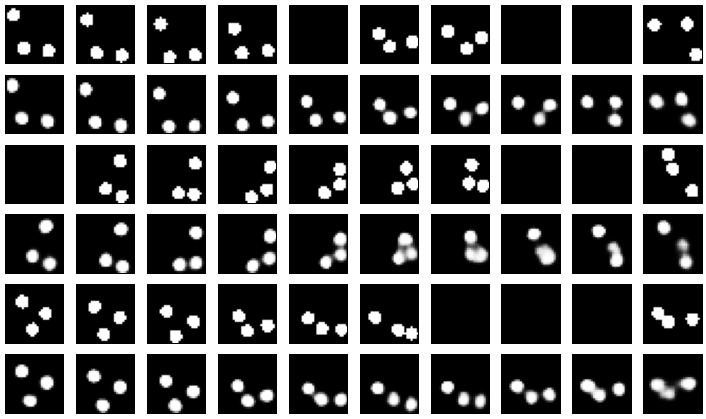
\includegraphics[scale=0.8]{whole_sequence_bouncingBalls}
%		\caption{Rekonstruktion der \emph{time series} mittels VAE ohne Interpolation.}
%		\label{Abb:VAEohneInterpolbouncingBalls}
%	\end{figure}
%	\newpage

	%\begin{figure}
	%	\begin{minipage}[position=l]{0.33\textwidth}
	%		\begin{mdframed}[style=inner]
	%			\center{Modellinput\vspace{0.2cm}}
	%			
\includegraphics[scale=0.5]{Modellinput}
	%		\end{mdframed}
		%\end{minipage}
		%\begin{minipage}[position=r]{0.67\textwidth}
		%	\begin{mdframed}[style=inner]
		%		\center{Extrapolation\vspace{0.2cm}}
		%		\includegraphics[scale=0.499]{Reconstructions}
		%	\end{mdframed}
		%\end{minipage}
		%\caption{Groundtruth (jeweils obere Reihe) und Rekonstruktionen des ODE$^2$VAE %(untere Reihe) auf den Testdatensätzen von Rotating MNIST und Bouncing Balls. Wie %erwähnt erhält das Modell nur die ersten drei Bilder der \emph{time series}, um %Vorhersagen für die restlichen Zeitpunkte zu treffen.}
%	\end{figure}
	\subsubsection{Methode 3: ODE$^2$VAE}
		\begin{figure}[h!]
		\begin{minipage}{0.143\textwidth}
			\center{\small{Modellinput}\vspace{0.1cm}}
			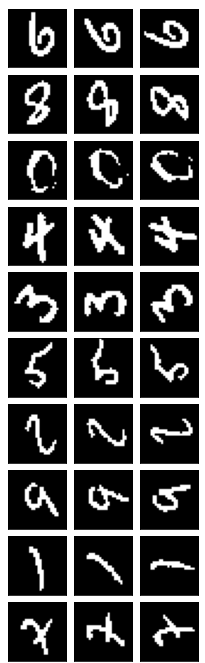
\includegraphics[scale=0.325]{MNISTorig1}
		\end{minipage}
		\begin{minipage}{0.346\textwidth}
			\center{Groundtruth\vspace{0.1cm}}
			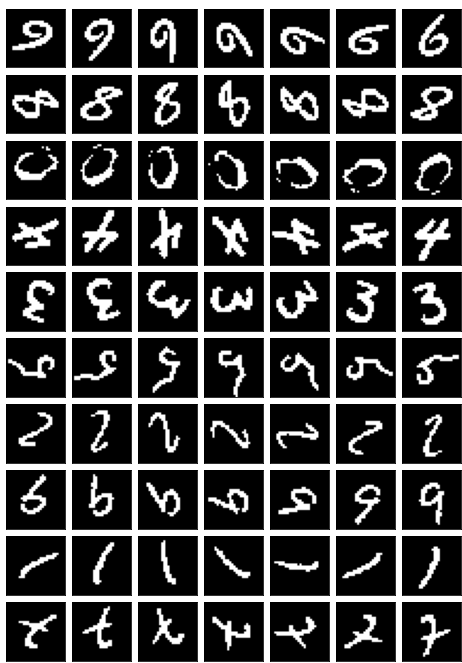
\includegraphics[scale=0.325]{MNISTorig2}
		\end{minipage}
		\begin{minipage}{0.5\textwidth}
		\center{Rekonstruktion und Extrapolation\vspace{0.1cm}}
			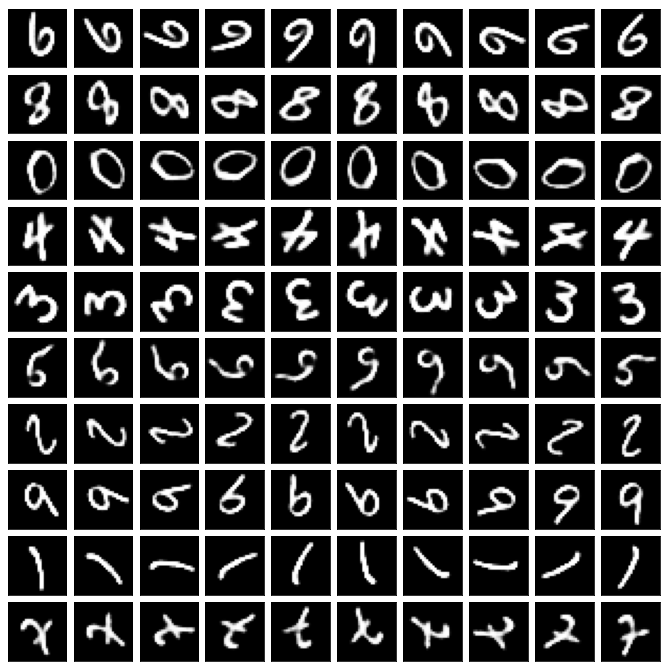
\includegraphics[scale=0.325]{MNISTrec}
		\end{minipage}
			\begin{minipage}{0.152\textwidth}
		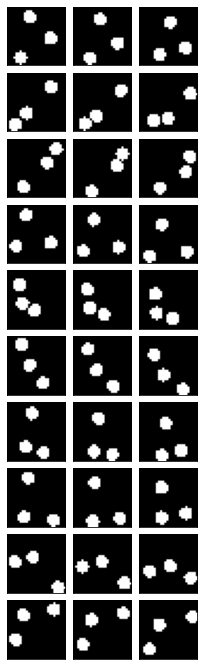
\includegraphics[scale=0.325]{bouncingBalls_ODEorig1}
		\end{minipage}
		\begin{minipage}{0.35\textwidth}
			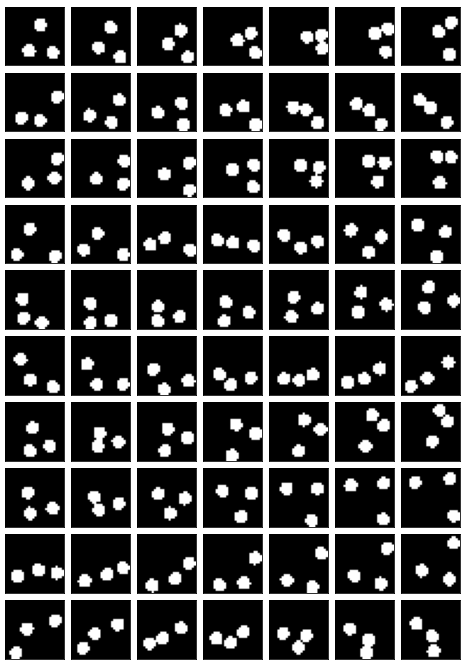
\includegraphics[scale=0.325]{bouncingBalls_ODEorig2}
		\end{minipage}
		\begin{minipage}{0.5\textwidth}
			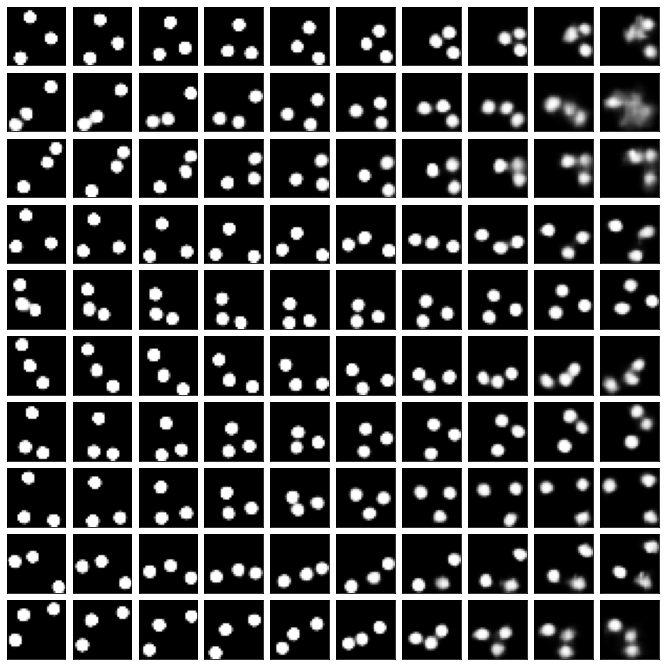
\includegraphics[scale=0.325]{bouncingBalls_ODE}
		\end{minipage}
		\end{figure}
	Auf diesen Abbildungen sind die Rekonstruktionen eines ODE$^2$VAE, auf den Datensätzen rotatingMNIST und bouncingBalls zu erkennen. Das Modell wurde für 40 Epochen auf einem unbeschädigten Datensatz trainiert und erhält zum anfertigen der Rekonstruktionen aber nur die ersten drei Bilder der time series. 
	Dieser Modellinput ist ganz links abgebildet. Daneben ist zum besseren einordnen der Ergebnisse die Groundtruth zu sehen, die das Modell zwar nicht sieht, von ihm aber bei einer perfekten Vorhersage aus den drei Inputdaten errechnet werden soll. Rechts ist schließlich die Rekonstruktion des Modellinputs und ab dem vierten Frame die Extrapolation zu erkennen. Wie man gut sehen kann ist die Modellperformance auf dem Datensatz rotatingMNIST hervorragend, während auf  bouncingBalls, der chaotischen Natur des Datensatzes geschuldet, auch einige Vorhersagen in den hinteren Frames nicht so gut aussehen. Dies dürfte daran liegen, dass sich anfänglich kleine Fehler in der Vorhersage mit fortlaufender Zeit immer weiter verschlimmern. \\
	Wir vermuten deswegen, dass das Modell davon profitieren könnte die Priorverteilung beispielsweise durch Inverse Autoregressive Flow von einer Normalverteilung zu einer aussagekräftigeren Verteilung zu transformieren. So könnte sicher gestellt werden, dass die Startposition sehr genau encodiert wird, was einem aufsummieren von Fehlern entgegenwirken würde.
	Dennoch von allen Methoden liefert dieses Modell auf den Datensätzen bereits auch so die besten Ergebnisse. Sollen nur ein oder zwei Frames rekonstruiert werden und sind die vorherigen drei Frames bekannt ist eine Rekonstruktion annährend fehlerfrei. 
	\begin{figure}[h!]
		\begin{minipage}[position=l]{0.5\textwidth}
			\begin{mdframed}[style=inner]
				\center{Modellinput\vspace{0.2cm}}
				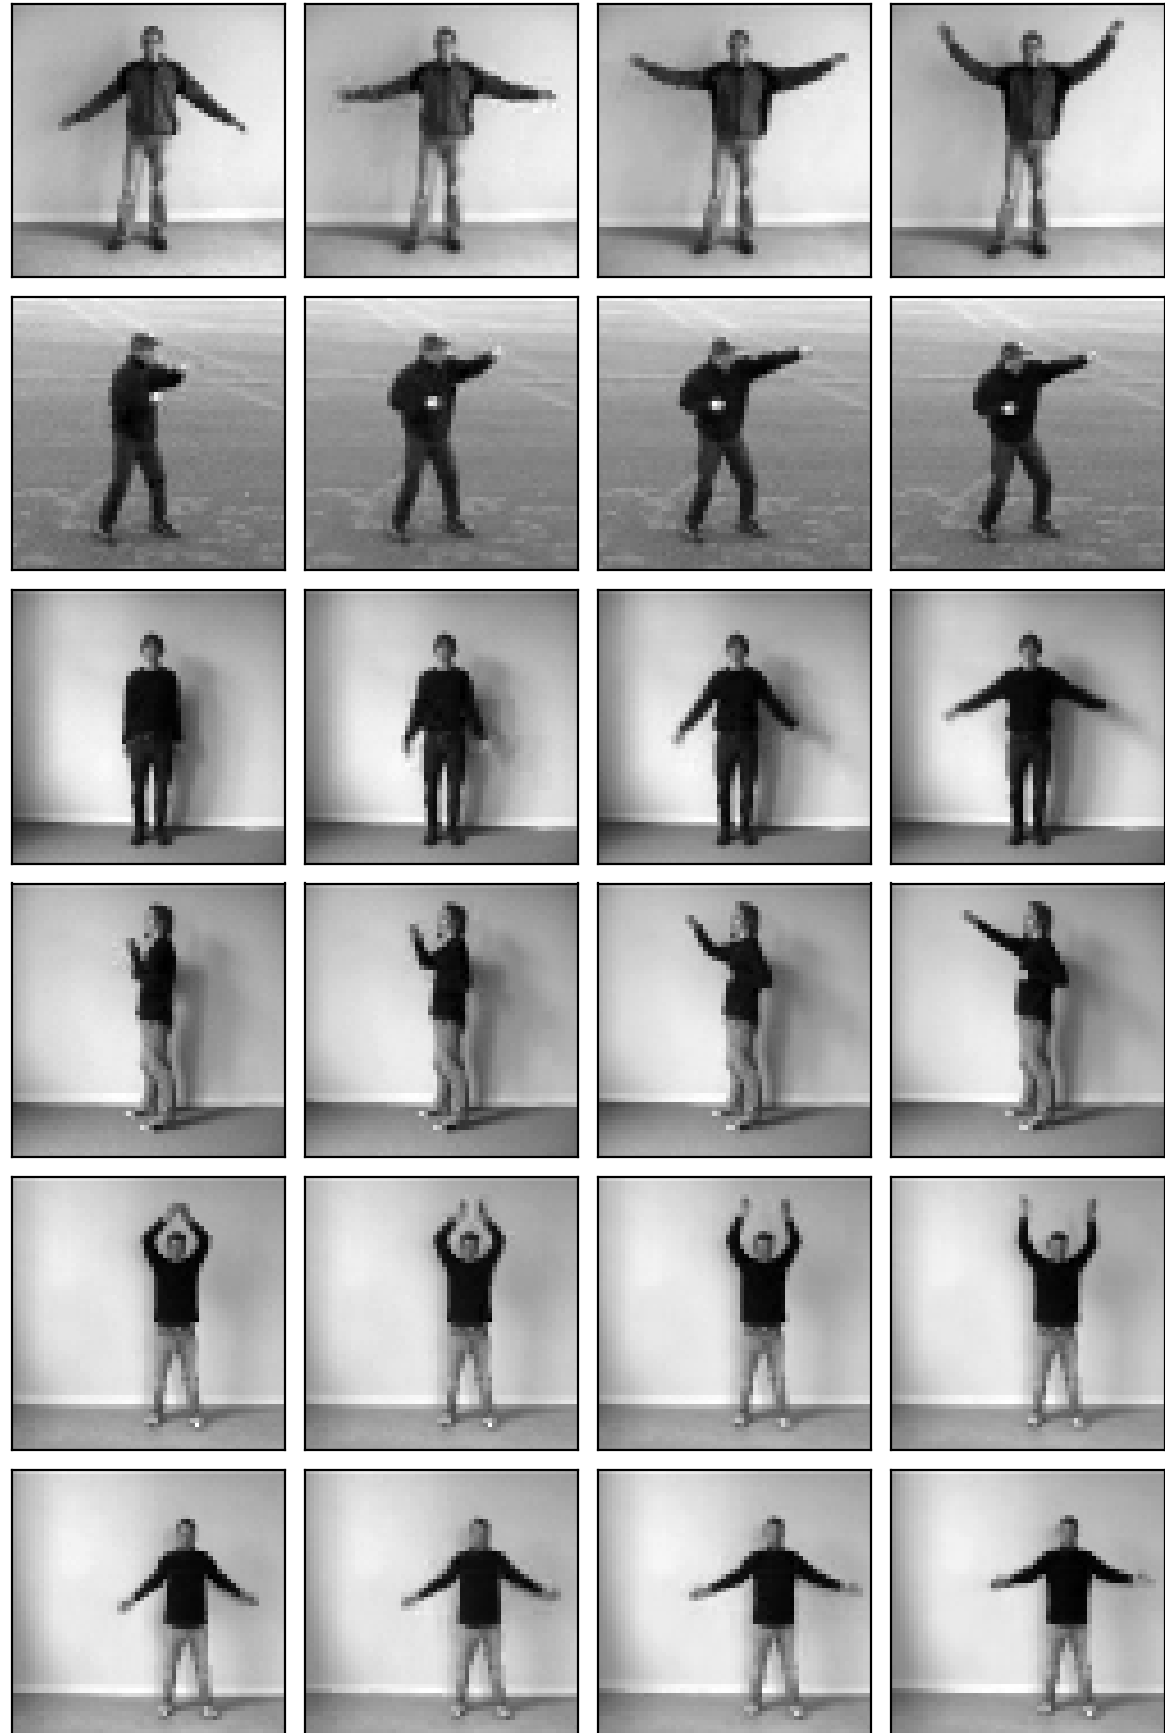
\includegraphics[scale=0.47]{movies_input}
			\end{mdframed}
		\end{minipage}
		\begin{minipage}[position=r]{0.5\textwidth}
			\begin{mdframed}[style=inner]
				\center{Extrapolation\vspace{0.2cm}}
				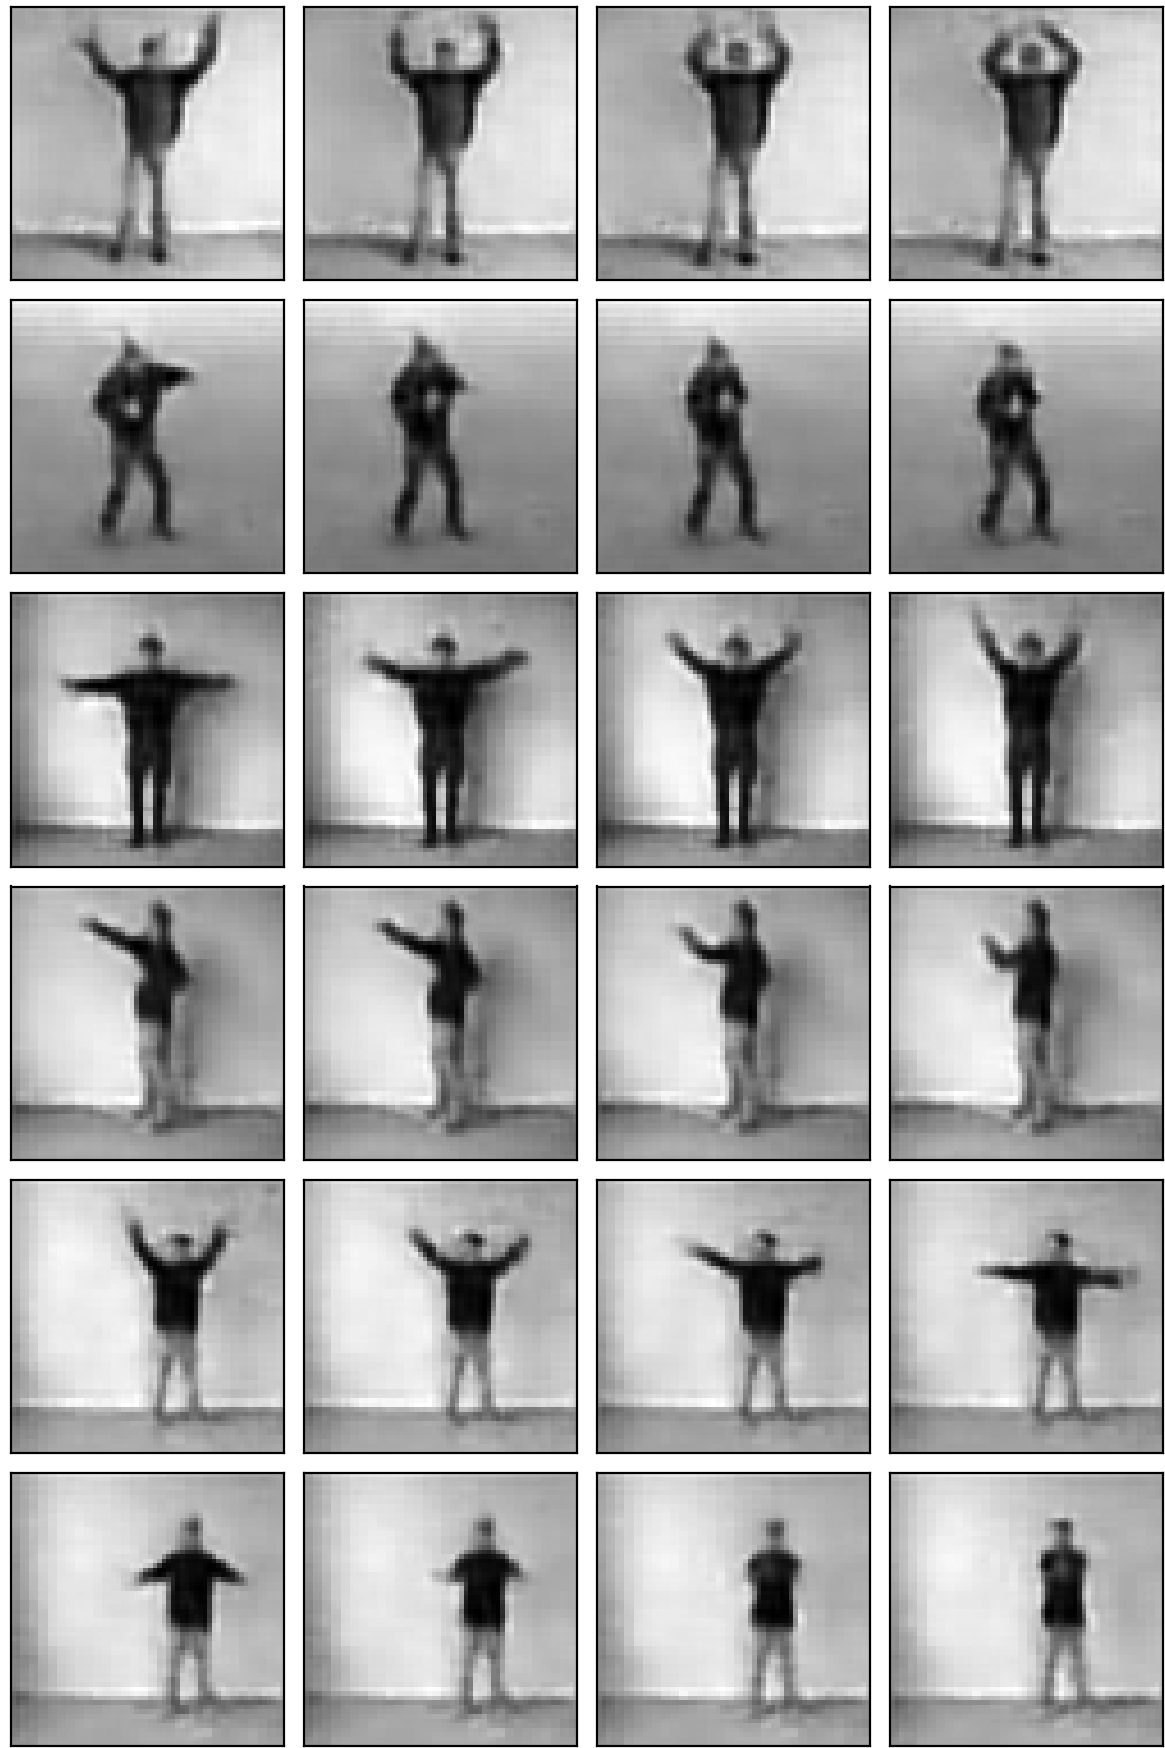
\includegraphics[scale=0.47]{movies_extrapolation}
			\end{mdframed}
		\end{minipage}
	\end{figure}
	Auf dem Datensatz AVI-Motion werden ebenfalls gute Ergebnisse erzielt. Die Bewegungen werden vom Modell gut vervollständigt, wir haben im Gegensatz zu den anderen Datensätzen dem Modell zur Bestimmung von $\mathbf{v}_0$ jedoch vier Bilder gezeigt. Die Extrapolation ist zwar etwas unscharf, könnte aber durch das Training von beispielsweise Adversarial Variational Autoencodern weiter an Qualität gewinnen. 
	
	
	\newpage
	\subsubsection{Methode 4: SDE$^n$VAE}
	Für den SDE-Ball-Datensatz erhalten wir nach 10 Epochen die folgenden Ergebnisse:\\
	\\
	TODO
	\\
	Für die Verlustfunktion haben wir dabei festgestellt, dass die Verlust-Gewichtung
	\begin{align*}
	& 20 \, L_r + 3 \, L_{lr} + 10 \, L_{lp} + 1 \, L_{cv}
	\end{align*}
	recht gut funktioniert.
	
	
	
	
	
	\newpage

	\begin{table}[htb]
		\begin{center}
			\begin{tabular}{p{4cm}>{\centering\arraybackslash}p{1.6cm}>{\centering\arraybackslash}p{2.5cm}>{\centering\arraybackslash}p{2.5cm}>{\centering\arraybackslash}p{2cm}>{\centering\arraybackslash}p{1.5cm}}\toprule
				\textbf{\ }	&\textbf{Vanilla-}\newline\textbf{VAE}	&\textbf{\ \ Latente}\newline\textbf{Interpolation}
				&\textbf{alternativer}\newline\textbf{ODE$^2$VAE}
				&\textbf{ODE$^2$VAE}
				&\textbf{SDE-}\newline\textbf{VAE} \\

				\textbf{Rekonstruktionen} \newline \textbf{in stetiger Zeit}& $\times$	& $\checkmark$ &$\times$ & $\checkmark$	& \\
				\textbf{Beobachtungs-}\newline\textbf{zeitpunkte können}\newline \textbf{unregelmäßig sein}	& $\times$	&  $\checkmark$ & $\times$ &$\checkmark$	& \\
				\textbf{Extrapolation}	& $\times$	& $(\checkmark)$ & $\checkmark$ & $\checkmark$	& \\
				\textbf{Trainingsdatensatz} \newline\textbf{mit fehlenden} \newline\textbf{Bildern möglich} 	& $\times$	& $\checkmark$ & $(\checkmark)$ & $(\checkmark)$	& \\
				\bottomrule
			\end{tabular}
		\end{center}
	\end{table}
	\newpage
	\section[Modellstrukturen]{Modellstrukturen}
	Diese Modellstruktur haben wir für die Implementierung des Vanilla-VAE's verwendet. Als Input dient hier die gesamte Videosequenz. Falls nur ein
	einzelnes Frame betrachtet werden soll, (z.B. auf dem normalen MNIST-Datensatz oder für lineare Interpolation) muss im Input-Layer des Encoders und im Output-Layer des Decoders die Channelsize von 10 auf 1 reduziert werden.

	\begin{table}[htb]
		\small
		\begin{center}
			\begin{tabular}{llcccc}
				\toprule
				\toprule
				\textbf{\ }	&\textbf{Encoder}	&\textbf{Outputgröße} &\textbf{Parameter} &\textbf{Fenstergröße} &\textbf{Aktivierung}\\
				\midrule
				\textbf{1.}	&Input-Layer	& (28, 28, 10)		& 0		& - 			&- \\
				\textbf{2.}	&Conv2D 		& (28, 28, 32)		& 2912	& 3 $\times$ 3; padding	&relu \\
				\textbf{3.}	&Max-Pooling2D	& (14, 14, 32)		& 0		& 2 $\times$ 2	&- \\
				\textbf{4.}	&Conv2D			& (12, 12, 64)		& 18496	& 3 $\times$ 3	&relu \\
				\textbf{5.}	&Max-Pooling2D	& (6, \ \ 6, \ 64)	& 0		& 2 $\times$ 2 	&- \\
				\textbf{6.}	&Conv2D		& (4, \ \ 4,  128)	& 73856	& 3 $\times$ 3 	&relu \\
				\textbf{7.}	&Flatten		& 2048				& 0		& - 			&- \\
				\textbf{8.}	&Dense-Layer			& 256				& 262272	& - 			&relu \\
				\textbf{9.}	&Dense-Layer 			& 20 + 20				& 10280	& - 			&- \\
				\textbf{10.}	&Split-Layer	($\boldsymbol{\mu}, \log\boldsymbol{\sigma}$)	& (20, 20)				& 0	& - 			&- \\
				\textbf{11.}&$\mathbf{z}=\boldsymbol{\mu}+\boldsymbol{\epsilon}\cdot\exp(\log\boldsymbol{\sigma})$		& 20				& 0	& - 			&-\\
				\bottomrule
				\toprule
				\textbf{\ }	&\textbf{Decoder}	&\textbf{Outputgröße} &\textbf{Parameter} &\textbf{Fenstergröße} &\textbf{Aktivierung}\\
				\midrule
				\textbf{1.}	&Input-Layer	& 20		& 0		& - 			&- \\
				\textbf{2.}	&Dense-Layer 			& 256		& 5376	& -				&relu \\
				\textbf{3.}	&Dense-Layer			& 2048		& 526336& -				&relu \\
				\textbf{4.}	&Reshape-Layer		& (4, \ \ 4,  128)	& 0		& -		&- \\
				\textbf{5.}	&Conv2DTranspose& (6, \ \ 6, \ 64)	& 73792	& 3 $\times$ 3 	&relu \\
				\textbf{6.}	&Up-Sampling2D	& (12, 12, \ 64)	& 0		& 2 $\times$ 2 	&- \\
				\textbf{7.}	&Conv2DTranspose& (14, 14, \ 32)	& 18464		& 3 $\times$ 3 			&relu \\
				\textbf{8.}	&Up-Sampling2D	& (28, 28, \ 32)	& 0	& 2 $\times$ 2 			&- \\
				\textbf{9.}	&Conv2DTranspose& (28, 28,\ \ 10)	& 5130  	& 3 $\times$ 3; padding 			&sigmoid \\
				\bottomrule
				\bottomrule
			\end{tabular}
		\end{center}
	\end{table}
	\newpage
	Die Modellstruktur des ODE$^2$VAE für die Datensätze rotatingMNIST und bouncingBalls. Im ODE-Net verwenden wir als Aktivierungsfunktion den
	Tangens hyperbolicus, da die ReLu-Funktion zum Modellieren von Differentialgleichungen, aufgrund relu$'(x)=0$, ungeeignet ist.
	\begin{table}[htb!]
		\footnotesize
		\begin{center}
			\begin{tabular}{llcccc}
				\toprule
				\toprule
				\textbf{\ }	&\textbf{Positionencoder}	&\textbf{Outputgröße} &\textbf{Parameter} &\textbf{Fenstergröße} &\textbf{Aktivierung}\\
				\midrule
				\textbf{1.}	&Input-Layer	& (28, 28, \ 1)		& 0		& - 			&- \\
				\textbf{2.}	&Conv2D 		& (28, 28, 32)		& 320	& 3 $\times$ 3; padding	&relu \\
				\textbf{3.}	&Max-Pooling2D	& (14, 14, 32)		& 0		& 2 $\times$ 2	&- \\
				\textbf{4.}	&Conv2D			& (12, 12, 64)		& 18496	& 3 $\times$ 3	&relu \\
				\textbf{5.}	&Max-Pooling2D	& (6, \ \ 6, \ 64)	& 0		& 2 $\times$ 2 	&- \\
				\textbf{6.}	&Conv2D		& (4, \ \ 4,  128)	& 73856	& 3 $\times$ 3 	&relu \\
				\textbf{7.}	&Flatten		& 2048				& 0		& - 			&- \\
				\textbf{8.}	&Dense-Layer			& 256				& 262272	& - 			&relu \\
				\textbf{9.}	&Dense-Layer 			& 20 + 20				& 10280	& - 			&- \\
				\textbf{10.}	&Split-Layer	($\boldsymbol{\mu}, \log\boldsymbol{\sigma}$)	& (20, 20)				& 0	& - 			&- \\
				\textbf{11.}&$\mathbf{s}=\boldsymbol{\mu}+\boldsymbol{\epsilon}\cdot\exp(\log\boldsymbol{\sigma})$		& 20				& 0	& - 			&-\\
				\bottomrule
				\toprule
				\textbf{\ }	&\textbf{Velocityencoder}	&\textbf{Outputgröße} &\textbf{Parameter} &\textbf{Fenstergröße} &\textbf{Aktivierung}\\
				\midrule
				\textbf{1.}	&Input-Layer	& (28, 28, \ 3)		& 0		& - 			&- \\
				\textbf{2.}	&Conv2D 		& (28, 28, 32)		& 896	& 3 $\times$ 3; padding	&relu \\
				\textbf{3.}	&Max-Pooling2D	& (14, 14, 32)		& 0		& 2 $\times$ 2	&- \\
				\textbf{4.}	&Conv2D			& (12, 12, 64)		& 18496	& 3 $\times$ 3	&relu \\
				\textbf{5.}	&Max-Pooling2D	& (6, \ \ 6, \ 64)	& 0		& 2 $\times$ 2 	&- \\
				\textbf{6.}	&Conv2D		& (4, \ \ 4,  128)	& 73856	& 3 $\times$ 3 	&relu \\
				\textbf{7.}	&Flatten		& 2048				& 0		& - 			&- \\
				\textbf{8.}	&Dense-Layer			& 256				& 262272	& - 			&relu \\
				\textbf{9.}	&Dense-Layer 			& 20 + 20				& 10280	& - 			&- \\
				\textbf{10.}	&Split-Layer	($\boldsymbol{\mu}, \log\boldsymbol{\sigma}$)	& (20, 20)				& 0	& - 			&- \\
				\textbf{11.}&$\mathbf{v}=\boldsymbol{\mu}+\boldsymbol{\epsilon}\cdot\exp(\log\boldsymbol{\sigma})$		& 20				& 0	& - 			&-\\
				\toprule
				\textbf{\ } &Concatenate $\mathbf{z}=(\mathbf{s},\mathbf{v})$& (2, 20) & 0 & - & -\\
				\bottomrule
				\toprule
				\textbf{\ }	&\textbf{ODE-Net}	&\textbf{Outputgröße} &\textbf{Parameter} &-  &\textbf{Aktivierung}\\
				\midrule
				\textbf{1.}	&Input-Layer	& (2, 20)		& 0		&-	&- \\
				\textbf{2.}	&Flatten	 	& 40			& 0		&-	&- \\
				\textbf{3.}	&Dense-Layer			& 100			& 4100	&-	&tanh \\
				\textbf{4.}	&Dense-Layer			& 100			& 10100	&-	&tanh \\
				\textbf{5.}	&Dense-Layer			& 20			& 2020	&-	& \\
				\bottomrule
				\toprule
				\textbf{\ }	&\textbf{Decoder}	&\textbf{Outputgröße} &\textbf{Parameter} &\textbf{Fenstergröße} &\textbf{Aktivierung}\\
				\midrule
				\textbf{1.}	&Input-Layer	& 20		& 0		& - 			&- \\
				\textbf{2.}	&Dense-Layer 			& 256		& 5376	& -				&relu \\
				\textbf{3.}	&Dense-Layer			& 2048		& 526336& -				&relu \\
				\textbf{4.}	&Reshape-Layer		& (4, \ \ 4,  128)	& 0		& -		&- \\
				\textbf{5.}	&Conv2DTranspose& (6, \ \ 6, \ 64)	& 73792	& 3 $\times$ 3 	&relu \\
				\textbf{6.}	&Up-Sampling2D	& (12, 12, \ 64)	& 0		& 2 $\times$ 2 	&- \\
				\textbf{7.}	&Conv2DTranspose& (14, 14, \ 32)	& 18464		& 3 $\times$ 3 			&relu \\
				\textbf{8.}	&Up-Sampling2D	& (28, 28, \ 32)	& 0	& 2 $\times$ 2 			&- \\
				\textbf{9.}	&Conv2DTranspose& (28, 28,\ \ \ 1)	& 513  	& 3 $\times$ 3; padding 			&sigmoid \\
				\bottomrule
				\bottomrule
			\end{tabular}
		\end{center}
	\end{table}
	\newpage
	Die Modellstruktur des ODE$^2$VAE für den Datensatz AVI-Motion.
	\begin{table}[htb!]
		\footnotesize
		\begin{center}
			\begin{tabular}{llcccc}
				\toprule
				\toprule
				\textbf{\ }	&\textbf{Positionencoder}	&\textbf{Outputgröße} &\textbf{Parameter} &\textbf{Fenstergröße} &\textbf{Aktivierung}\\
				\midrule
				\textbf{1.}	&Input-Layer	& (60, 60, \ 1)		& 0		& - 			&- \\
				\textbf{2.}	&Conv2D 		& (56, 56, 32)		& 823	& 5 $\times$ 5	&relu \\
				\textbf{3.}	&Max-Pooling2D	& (14, 14, 32)		& 0		& 2 $\times$ 2	&- \\
				\textbf{3.}	&Conv2D 		& (28, 28, 32)		& 9248	& 3 $\times$ 3; padding	&relu \\
				\textbf{4.}	&Max-Pooling2D	& (14, 14, 32)		& 0		& 2 $\times$ 2	&- \\
				\textbf{5.}	&Conv2D			& (12, 12, 64)		& 18496	& 3 $\times$ 3	&relu \\
				\textbf{6.}	&Max-Pooling2D	& (6, \ \ 6, \ 64)	& 0		& 2 $\times$ 2 	&- \\
				\textbf{7.}	&Conv2D			& (5, \ \ 5,  128)	& 32896	& 2 $\times$ 2 	&relu \\
				\textbf{8.}	&Flatten		& 3200				& 0		& - 			&- \\
				\textbf{9.}	&Dense-Layer	& 384				&1229184& - 			&relu \\
				\textbf{10.}&Dense-Layer 	& 30 + 30			& 23100	& - 			&- \\
				\textbf{11.}&Split-Layer($\boldsymbol{\mu}, \log\boldsymbol{\sigma}$)   & (30, 30)				& 0	& - 			&- \\
				\textbf{12.}&$\mathbf{s}=\boldsymbol{\mu}+\boldsymbol{\epsilon}\cdot\exp(\log\boldsymbol{\sigma})$	& 30				& 0	& - 			&-\\
				\bottomrule
				\toprule
				\textbf{\ }	&\textbf{Velocityencoder}	&\textbf{Outputgröße} &\textbf{Parameter} &\textbf{Fenstergröße} &\textbf{Aktivierung}\\
				\midrule
				\textbf{1.}	&Input-Layer	& (60, 60, \ 4)		& 0		& - 			&- \\
				\textbf{2.}	&Conv2D 		& (56, 56, 64)		& 6464	& 5 $\times$ 5	&relu \\
				\textbf{3.}	&Max-Pooling2D	& (14, 14, 64)		& 0		& 2 $\times$ 2	&- \\
				\textbf{3.}	&Conv2D 		& (28, 28, 64)		& 36928	& 3 $\times$ 3; padding	&relu \\
				\textbf{4.}	&Max-Pooling2D	& (14, 14, 64)		& 0		& 2 $\times$ 2	&- \\
				\textbf{5.}	&Conv2D			& (12, 12, 128)		& 73856 & 3 $\times$ 3	&relu \\
				\textbf{6.}	&Max-Pooling2D	& (6, \ \ 6, \ 128)	& 0		& 2 $\times$ 2 	&- \\
				\textbf{7.}	&Conv2D		& (5, \ \ 5,  256)		& 131328& 2 $\times$ 2 	&relu \\
				\textbf{8.}	&Flatten		& 6400				& 0		& - 			&- \\
				\textbf{9.}	&Dense-Layer			& 640				& 4096640	& - 			&relu \\
				\textbf{10.}	&Dense-Layer 			& 30 + 30				& 38460	& - 			&- \\
				\textbf{11.}	&Split-Layer	($\boldsymbol{\mu}, \log\boldsymbol{\sigma}$)	& (30, 30)				& 0	& - 			&- \\
				\textbf{12.}&$\mathbf{v}=\boldsymbol{\mu}+\boldsymbol{\epsilon}\cdot\exp(\log\boldsymbol{\sigma})$		& 30				& 0	& - 			&-\\
				\toprule
				\textbf{\ } &Concatenate $\mathbf{z}=(\mathbf{s},\mathbf{v})$& (2, 30) & 0 & - & -\\
				\bottomrule
				\toprule
				\textbf{\ }	&\textbf{ODE-Net}	&\textbf{Outputgröße} &\textbf{Parameter} &- &\textbf{Aktivierung}\\
				\midrule
				\textbf{1.}	&Input-Layer	& (2, 30)		& 0		&-	&- \\
				\textbf{2.}	&Flatten	 	& 60			& 0		&-	&- \\
				\textbf{3.}	&Dense-Layer			& 120			& 7320	&-	&tanh \\
				\textbf{4.}	&Dense-Layer			& 120			& 14520	&-	&tanh \\
				\textbf{5.}	&Dense-Layer			& 30			& 3630	&-	&- \\
				\bottomrule
				\toprule
				\textbf{\ }	&\textbf{Decoder}	&\textbf{Outputgröße} &\textbf{Parameter} &\textbf{Fenstergröße} &\textbf{Aktivierung}\\
				\midrule
				\textbf{1.}	&Input-Layer	& 20				& 0		& - 			&- \\
				\textbf{2.}	&Dense-Layer 	& 384				& 11904 & -				&relu \\
				\textbf{3.}	&Dense-Layer	& 3200				& 1232000& -				&relu \\
				\textbf{4.}	&Reshape-Layer	& (4, \ \ 4,  128)	& 0		& -		&- \\
				\textbf{5.}	&Conv2DTranspose& (6, \ \ 6, \ 64)	& 32832	& 2 $\times$ 2 	&relu \\
				\textbf{6.}	&Up-Sampling2D	& (12, 12, \ 64)	& 0		& 2 $\times$ 2 	&- \\
				\textbf{7.}	&Conv2DTranspose& (14, 14, \ 32)	& 18464		& 3 $\times$ 3 			&relu \\
				\textbf{8.}	&Up-Sampling2D	& (28, 28, \ 32)	& 0	& 2 $\times$ 2 			&- \\
				\textbf{9.}	&Conv2DTranspose& (28, 28,\ \ 32)	& 16416  	& 3 $\times$ 3; padding 			&relu \\
				\textbf{10.}&Up-Sampling2D	& (56, 56, \ 32)	& 0	& 2 $\times$ 2 			&- \\
				\textbf{11.}&Conv2DTranspose& (60, 60,\ \ \ 1)	& 801  	& 5 $\times$ 5 &sigmoid \\
				\bottomrule
				\bottomrule
			\end{tabular}
		\end{center}
	\end{table}
	\newpage
	\textbf{To-Do: SDE-VAE Modellstruktur}\\
	\begin{table}[htb]
		\small
		\begin{center}
			\begin{tabular}{llcccc}
				\toprule
				\toprule
				\textbf{\ }	&\textbf{Encoder}	&\textbf{Outputgröße} &\textbf{Parameter} &\textbf{Fenstergröße} &\textbf{Aktivierung}\\
				\midrule
				\textbf{1.}	&Input-Layer	& (28, 28, 1)		& 0		& - 			&- \\
				\textbf{2.}	&Conv2D 		& (28, 28, 16)		& 160	& 3 $\times$ 3; padding	&relu \\
				\textbf{3.}	&Max-Pooling2D	& (14, 14, 16)		& 0		& 2 $\times$ 2	&- \\
				\textbf{4.}	&Conv2D			& (12, 12, 32)		& 4640	& 3 $\times$ 3	&relu \\
				\textbf{5.}	&Max-Pooling2D	& (6, \ \ 6, \ 32)	& 0		& 2 $\times$ 2 	&- \\
				\textbf{6.}	&Conv2D		& (4, \ \ 4,  64)	& 18496	& 3 $\times$ 3 	&relu \\
				\textbf{7.}	&Flatten		& 1024				& 0		& - 			&- \\
				\textbf{8.}	&Dense-Layer			& 128				& 131200	& - 			&relu \\
				\textbf{9.}	&Dense-Layer 			& d + d				& 2 d 129	& - 			&- \\
				\textbf{10.}	&Split-Layer	($\boldsymbol{\mu}, \log\boldsymbol{\sigma}$)	& (d, d)				& 0	& - 			&- \\
				\textbf{11.}&$\mathbf{z}=\boldsymbol{\mu}+\boldsymbol{\epsilon}\cdot\exp(\log\boldsymbol{\sigma})$		& d				& 0	& - 			&-\\
				\bottomrule
				\toprule
				\textbf{\ }	&\textbf{Decoder}	&\textbf{Outputgröße} &\textbf{Parameter} &\textbf{Fenstergröße} &\textbf{Aktivierung}\\
				\midrule
				\textbf{1.}	&Input-Layer	& d		& 0		& - 			&- \\
				\textbf{2.}	&Dense-Layer 			& 128		& (d+1)128	& -				&relu \\
				\textbf{3.}	&Dense-Layer			& 1024		& 132096& -				&relu \\
				\textbf{4.}	&Reshape-Layer		& (4, \ \ 4,  64)	& 0		& -		&- \\
				\textbf{5.}	&Conv2DTranspose& (6, \ \ 6, \ 32)	& 18464	& 3 $\times$ 3 	&relu \\
				\textbf{6.}	&Up-Sampling2D	& (12, 12, \ 32)	& 0		& 2 $\times$ 2 	&- \\
				\textbf{7.}	&Conv2DTranspose& (14, 14, \ 16)	& 4624		& 3 $\times$ 3 			&relu \\
				\textbf{8.}	&Up-Sampling2D	& (28, 28, \ 16)	& 0	& 2 $\times$ 2 			&- \\
				\textbf{9.}	&Conv2DTranspose& (28, 28,\ \ 1)	& 257  	& 3 $\times$ 3; padding 			&sigmoid \\
				\bottomrule
				\toprule
				\textbf{\ }	&\textbf{$\bmu$-Netz}	&\textbf{Outputgröße} &\textbf{Parameter} &\textbf{Fenstergröße} &\textbf{Aktivierung}\\
				\midrule
				\textbf{1.}	&Input-Layer	& (M,d)		& 0		& - 		&- \\
				\textbf{2.}	&Flatten		& M d				& 0		& - 			&- \\
				\textbf{3.}	&Dense-Layer			& 20 M		& (M d + 1) 20 M & -				&tanh \\
				\textbf{4.}	&Dense-Layer		& 20 M	& (20 M + 1) 20 M		& -		&- \\
				\textbf{5.}	&Dense-Layer& M d	& (20 M + 1) M d	& - 	&tanh \\
				\textbf{6.}	&Reshape-Layer		& (M, d)	& 0		& -		&- \\
				\bottomrule
				\toprule
				\textbf{\ }	&\textbf{$\bsig$-Netz}	&\textbf{Outputgröße} &\textbf{Parameter} &\textbf{Fenstergröße} &\textbf{Aktivierung}\\
				\midrule
				\textbf{1.}	&Input-Layer	& (M,d)		& 0		& - 			&- \\
				\textbf{2.}	&Flatten		& M d				& 0		& - 			&- \\
				\textbf{3.}	&Dense-Layer			& 20 M n		& (M d + 1) 20 M n& -				&tanh \\
				\textbf{4.}	&Dense-Layer		& 20 M n	& (20 M n + 1) 20 M n	& -		&- \\
				\textbf{5.}	&Dense-Layer& M d n	& (20 M d + 1) M d n	& - 	&tanh \\
				\textbf{6.}	&Reshape-Layer		& (M, d, n)	& 0		& -		&- \\
				\bottomrule
				\bottomrule
			\end{tabular}
		\end{center}
	\end{table}
	
	
	
	
	
	
	
	\newpage
	\section[Quellenangabe]{Quellenangabe}
	\begin{thebibliography}{9}
		\bibitem{vae}
		Diederik P. Kingma, Max Welling,
		\textit{Auto-Encoding Variational Bayes},
		2013,\\
		arXiv:1312.6114v10

		\bibitem{intvae}
		Diederik P. Kingma, Max Welling,
		\textit{An Introduction to Variational Autoencoders},
		2019,
		arXiv:1906.02691v3

		\bibitem{ode2vae}
		Çağatay Yıldız, Markus Heinonen, Harri Lähdesmäki,
		\textit{ODE$^{\ 2}$-VAE: Deep generative second order ODEs with Bayesian neural networks},
		2019,
		arXiv:1905.10994v2

		\bibitem{repara}
		https://gabrielhuang.gitbooks.io/machine-learning/content/reparametrization-trick.html

		\bibitem{tutvae}
		Carl Doersch,
		\textit{Tutorial on Variational Autoencoders},
		2016,\\
		arXiv:1606.05908,
		Ähnliche Grafik zu finden auf S.5

		\bibitem{matrix}
		Kaare B. Petersen, Michael S. Pedersen,
		\textit{The Matrix Cookbook},
		2012,
		http://matrixcookbook.com%, Verwendete Rechentricks auf S.43

		\bibitem{neuralode}
		Ricky T. Q. Chen, Yulia Rubanova, Jesse Bettencourt, David Duvenaud,\\
		\textit{Neural Ordinary Differential Equations},
		2019, arXiv:1806.07366v5

		\bibitem{ffjord}
		Will Grathwohl, Ricky T. Q. Chen, Jesse Bettencourt, Ilya Sutskever, David Duvenaud,
		\textit{FFJORD:  Free-Form Continous Dynamics for Scalable Reversible Generative Models}
		2018, arXiv:1810.01367v3

		\bibitem{Hutchin}
		http://blog.shakirm.com/2015/09/machine-learning-trick-of-the-day-3-hutchinsons-trick/

		\bibitem{PfaffiSkript}
		https://www.stochastik.uni-freiburg.de/professoren/pfaffelhuber/inhalte/2020zyklus

		\bibitem{ElastKol}
		https://en.wikipedia.org/wiki/Elastic\_collision

		\bibitem{Dataset}
		https://www.csc.kth.se/cvap/actions/
	\end{thebibliography}
\end{document}
